%!TEX TS-program = xetex 
%!TEX encoding = UTF-8 Unicode 
\documentclass[DIV=7, bibliography=totoc,version=first, twoside,open=left,titlepage,fleqn,numbers=noenddot,headinclude,%1headlines,%    
fontsize=10pt,footinclude,cleardoublepage=empty,abstract=false, % <--- obsolete, remove (todo)
draft=on]{scrreprt}
% ********************************************************************
% Development Stuff
% ********************************************************************
\listfiles
%\usepackage[l2tabu, orthodox, abort]{nag}
%\usepackage[warning, all]{onlyamsmath}

% Sync between editor and viewer
\synctex=1

% ********************************************************************
% Re-usable information
% ********************************************************************
\newcommand{\myTitle}{High Performance Computing on Graphic Processing Units\xspace}
\newcommand{\myDegree}{An Homage to The Elements of Typographic Style\xspace}
\newcommand{\myName}{Zvonko Krnjaji\'c\xspace}
\newcommand{\myProf}{Dr. Abbes Amira\xspace}
\newcommand{\myOtherProf}{Put name here\xspace}
\newcommand{\mySupervisor}{Dr. Abbes Amira\xspace}
\newcommand{\myFaculty}{Put data here\xspace}
\newcommand{\myDepartment}{Put data here\xspace}
\newcommand{\myUni}{\protect{Brunel University}\xspace}
\newcommand{\myLocation}{Gerlingen\xspace}
\newcommand{\myTime}{May/2009\xspace}
\newcommand{\myVersion}{Version 2.5\xspace}


\usepackage{dissertation}

% ********************************************************************
% Setup and Finetuning
%*******************************************************
\newlength{\abcd} % for ab..z string length calculation
\newcommand{\myfloatalign}{\centering} % how all the floats will be aligned
\setlength{\extrarowheight}{3pt} % increase table row height


%********************************************************************
% Hyphenation
%*******************************************************
%\hyphenation{put special hyphenation here}
\usepackage{layout}
%\usepackage[colorgrid, draft]{showframe}


\begin{document}
\layout*
%\printparam

\color{textcolor}

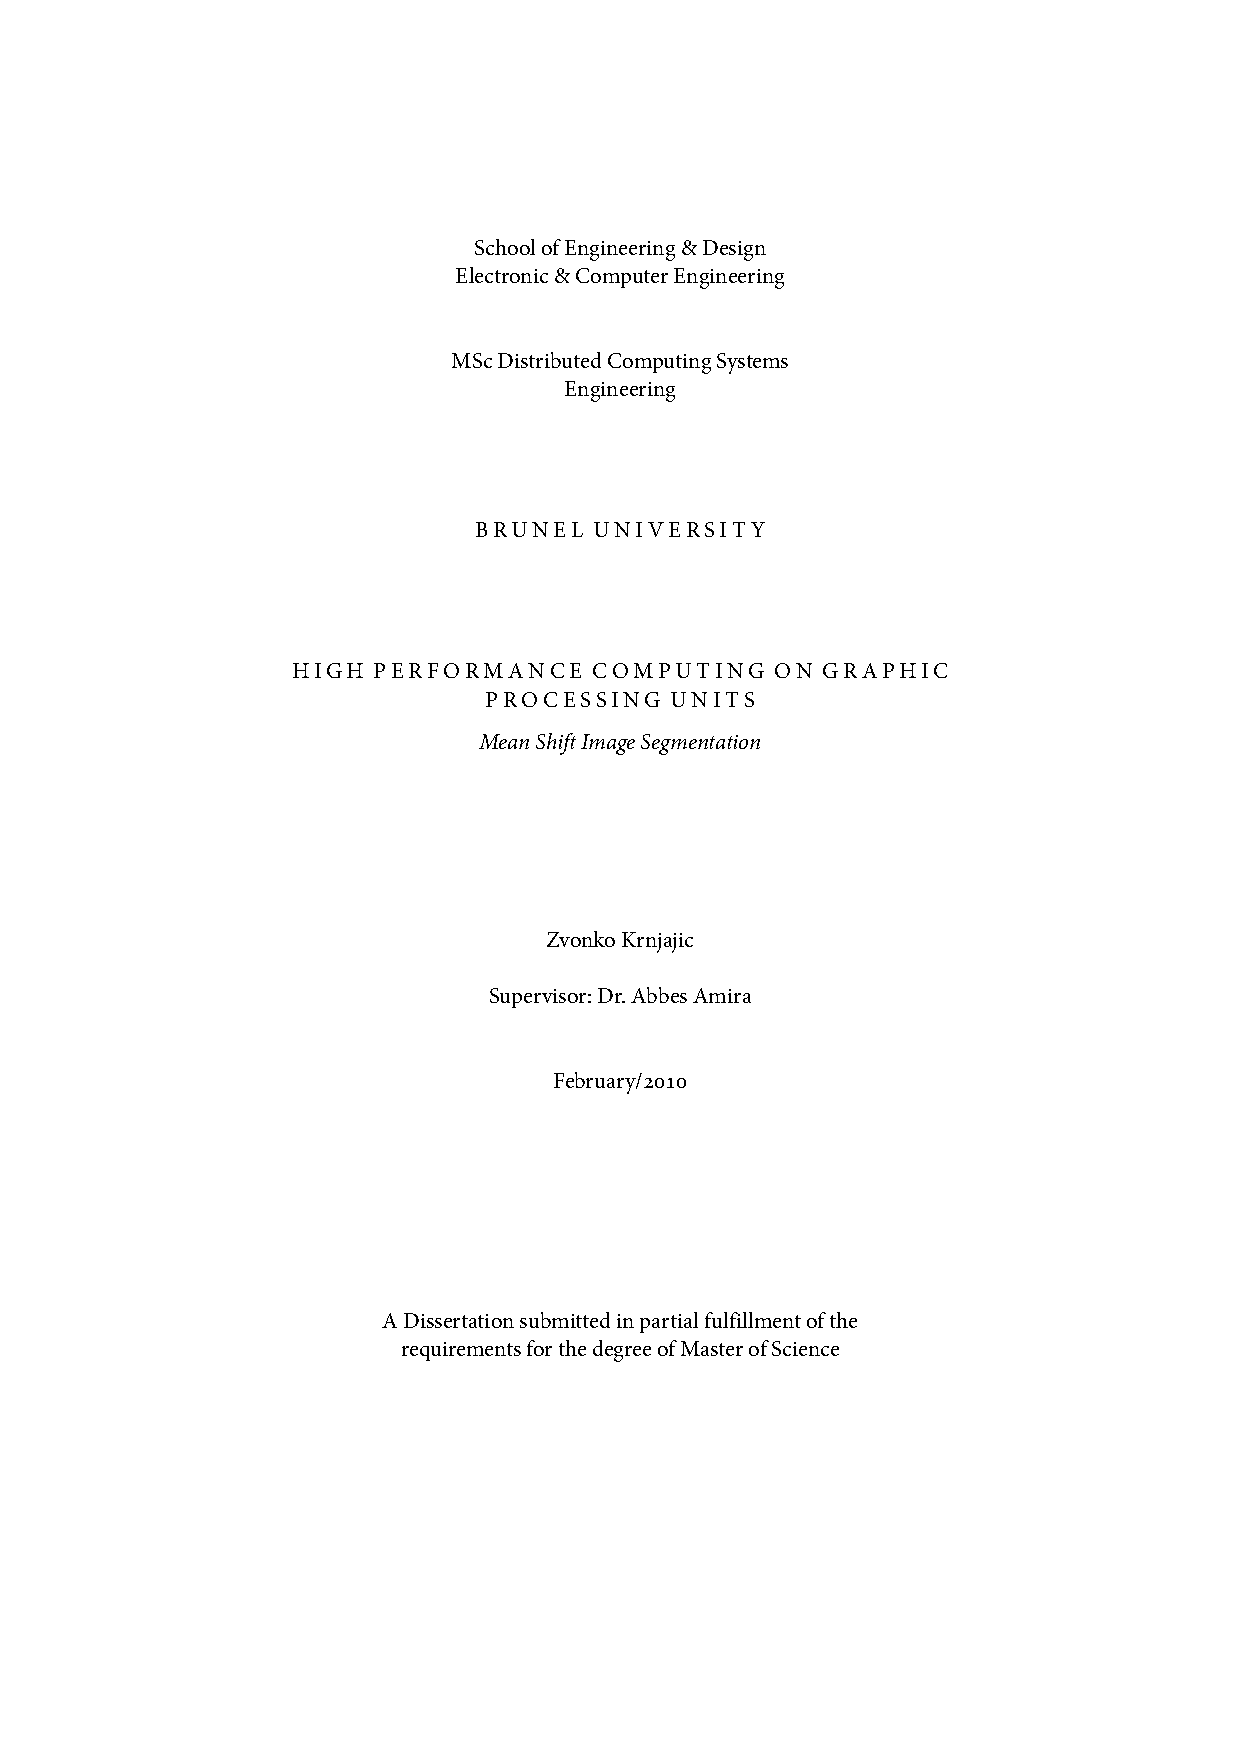
\includepdf{Frontcover.pdf}

\selectlanguage{american} % american ngerman
%\renewcommand*{\bibname}{new name}
%\setbibpreamble{}
\pagenumbering{roman}
\pagestyle{empty}

%*******************************************************************************
%\frontmatter
%*******************************************************************************
%Befehle für Symbole
%\newglossaryentry{symb:Pi}{name=$\pi$, description={Die Kreiszahl.}}
%\newglossaryentry{symb:Phi}{name=$\varphi$,description={Ein beliebiger Winkel.}}
\newglossaryentry{Pi}{name=$\pi$, description={Die Kreiszahl}}
\newglossaryentry{Phi}{name=$\varphi$, description={Ein beliebiger Winkel}}
\newglossaryentry{Performance}{name=Performance, description={Laufzeitanalyse}}



% Acronyms
\newacronym{GPGPU}{GPGPU}{General Purpose Computation on GPUs}
\newacronym{GPU}{GPU}{Graphic Processing Unit}
\newacronym{CPU}{CPU}{Central Processing Unit}
\newacronym{SIMD}{SIMD}{Single Instruction Multiple Data}
\newacronym{HPC}{HPC}{High Performance Computing}
\newacronym{CUDA}{CUDA}{Common Unified Device Architecture}
\newacronym{SM}{SM}{Streaming Multiprocessor}
\newacronym{GFLOP}{GFLOP}{Giga FLoating point Operations Per Second}
\newacronym{SDK}{SDK}{Software Development Kit}
\newacronym{API}{API}{Application Programming Interface}
\newacronym{EDISON}{EDISON}{Edge Detection and Image SegmentatiON System}
\newacronym{MISE}{MISE}{Mean Integrated Squared Error}
\newacronym{RGB}{RGB}{Red Green Blue}
\newacronym{HSV}{HSV}{Hue Saturation Value}
\newacronym{LUV}{Luv}{L* u* v*}
\newacronym{GHz}{GHz}{Giga Hertz}
\newacronym{USM}{USM}{Unified Shader Model}
\newacronym{ANSI}{ANSI}{American National Standards Institute}
\newacronym{ALU}{ALU}{Arithmetic Logic Unit}
\newacronym{GB}{GB}{Gigabyte}
\newacronym{GDDR3}{GDDR3}{Graphics Double Data Rate v3}
\newacronym{1D}{1D}{one-dimensional}
\newacronym{2D}{2D}{two-dimensional}
\newacronym{3D}{3D}{three-dimensional}
\newacronym{PCIE}{PCI-E}{Peripheral Component Interconnect Express}
\newacronym{RW}{RW}{read-write}
\newacronym{RO}{RO}{read-only}
\newacronym{DMA}{DMA}{Direct Memory Access}
\newacronym{KB}{KB}{Kilobyte}
\newacronym{SPMD}{SPMD}{Single Program Multiple Data}
%*******************************************************
% Titlepage
%*******************************************************
\begin{titlepage}
    \begin{center}
        \large  
		\vspace*{1cm}
		{School of Engineering \& Design}\\
		{Electronic \& Computer Engineering}\\
		\vspace{1.2cm}
		{MSc Distributed Computing Systems}\\
		{Engineering}\\
		\vspace{2cm}
		\huge
		{\myUni}\\
		\vspace{2.5cm}
		\Huge
		\begingroup
			\color{seccolor}{\myTitle}\\
			\textit{\large{Mean Shift Image Segmentation}} \\
		\endgroup	
		\vspace{4.5cm}
		\large
	\begin{flushleft}
		{Student's name: \myName 0631351}\\
		\vspace{0.5cm}
	   	{Signature of student: }\\
	 \end{flushleft}
		
		\vfill
%		\spacedlowsmallcaps{\myTime}\\
		
		\normalsize

    \end{center}
\end{titlepage}        

\thispagestyle{empty}
A Dissertation submitted in partial fulfillment\\
of the requirements for the degree of Master of Science


%\noindent\myName: \textit{\myTitle,} \myDegree, \textcopyright\ \myTime

\hfill

\vfill

%\bigskip
%
%\noindent\spacedlowsmallcaps{Supervisors}: \\
%\myProf \\
%\myOtherProf \\ 
%\mySupervisor
%
%\medskip
%
%\noindent\spacedlowsmallcaps{Location}: \\
%\myLocation
%
%\medskip
%
%\noindent\spacedlowsmallcaps{Time Frame}: \\
%\myTime

%*******************************************************
% Declaration
%*******************************************************
\refstepcounter{dummy}
\pdfbookmark[0]{Declaration}{declaration}
\chapter*{Declaration}
\thispagestyle{empty}
I have read and I understand the Dissertation guidelines on plagiarism and
cheating, and I certify that this submission fully complies with these 
guidelines.
\bigskip
 
\noindent\textit{\myLocation, \myTime}

\smallskip

\begin{flushright}
    \begin{tabular}{m{5cm}}
        \\ \hline
        \centering\myName \\
    \end{tabular}
\end{flushright}

%\cleardoublepage%*******************************************************
% Dedication
%*******************************************************
\thispagestyle{empty}
%\phantomsection 
\refstepcounter{dummy}
\pdfbookmark[1]{Dedication}{Dedication}

\vspace*{3cm}

\begin{center}
    \emph{Ohana} means family. \\
    Family means nobody gets left behind, or forgotten. \\ \medskip
    --- Lilo \& Stitch    
\end{center}

\medskip

\begin{center}
    Dedicated to the loving memory of Rudolf Miede. \\ \smallskip
    1939\,--\,2005
\end{center}
\cleardoublepage%*******************************************************
% Abstract
%*******************************************************
\chapter*{Abstract}
\renewcommand{\chapterpagestyle}{empty}
% Motivation: Why do we care about the problem and the results? If the 
% isn't obviously "interesting" it might be better to put motivation first; 
% but if your work is incremental progress on a problem that is widely 
% recognized as important, then it is probably better to put the problem 
% statement first to indicate which piece of the larger problem you are breaking
% off to work on. This section should include the importance of your work, the 
% difficulty of the area, and the impact it might have if successful.#
Today's \glspl{GPU} are not only good for gaming and graphics processing their
highly parallel structure is predestined for a range of complex algorithms. They
offer a tremendous memory bandwidth and computational power. Contrary to
\glspl{CPU}, \glspl{GPU} are accelerating quickly and advancing at incredible
rates in terms of absolute transistor count. Implementing a massively parallel,
unified shader design, its flexibility and programmability makes the \gls{GPU}
an attractive platform for general purpose computation. Recent improvements in
its programmability, especially high level languages (like C or C++), %
\glspl{GPU} have attracted developers to exploit the computational power of the
hardware for general purpose computing.

%* Problem statement: What problem are you trying to solve? What is the scope of your work (a generalized approach, or for a specific situation)? Be careful not to use too much jargon. In some cases it is appropriate to put the problem statement before the motivation, but usually this only works if most readers already understand why the problem is important.
Several \gls{GPU} programming interfaces and \glspl{API} represent a graphics
centric programming model to developers that is exported by a device driver and
tuned for real time graphics and games. Porting non-graphics applications to
graphics hardware means developing against the graphics programming model. Not
only the difficulties of the unusual graphics centric programming model but also
limitations of the hardware makes development of non-graphics applications a
tedious task.

%* Approach: How did you go about solving or making progress on the problem? Did
%you use simulation, analytic models, prototype construction, or analysis of
%field data for an actual product? What was the extent of your work (did you look
%at one application program or a hundred programs in twenty different programming
%languages?) What important variables did you control, ignore, or measure?
Therefore {\slcsmallcaps{NVIDIA}} Corporation developed the \gls{CUDA} that is a fundamentally new
computing architecture that simplifies software development by using the
standard C language. Using \gls{CUDA} this thesis will show on the basis of an
massively parallel application in which extent \glspl{GPU} are suitable for
general purpose computation. Special attention is paid to performance,
computational concepts, efficient data structures and program optimization.

%* Results: What's the answer? Specifically, most good computer architecture papers conclude that something is so many percent faster, cheaper, smaller, or otherwise better than something else. Put the result there, in numbers. Avoid vague, hand-waving results such as "very", "small", or "significant." If you must be vague, you are only given license to do so when you can talk about orders-of-magnitude improvement. There is a tension here in that you should not provide numbers that can be easily misinterpreted, but on the other hand you don't have room for all the caveats.
The result of this work is the demonstration of feasibility of \gls{GPGPU}. It
will show that \glspl{GPU} are capable of accelerating specific applications by
an order of magnitude.

%* Conclusions: What are the implications of your answer? Is it going to change the world (unlikely), be a significant "win", be a nice hack, or simply serve as a road sign indicating that this path is a waste of time (all of the previous results are useful). Are your results general, potentially generalizable, or specific to a particular case?
This work will represent a general guideline for suggestions and hints as 
well as drawbacks and obstacles when porting applications to \glspl{GPU}.


\vfill
\cleardoublepage%*******************************************************
% Acknowledgments
%*******************************************************
\pdfbookmark[1]{Acknowledgments}{acknowledgments}
\thispagestyle{empty}

\begingroup
\section*{Acknowledgments}
Put  acknowledgments here.

\endgroup





\pagenumbering{arabic}
\pagestyle{scrheadings}
\cleardoublepage%*******************************************************
% Table of Contents
%*******************************************************
\renewcommand{\chapterpagestyle}{empty}
\renewcommand{\contentsname}{Content Overview}
	
\setcounter{tocdepth}{2}
\tableofcontents%

\cleardoublepage


%*******************************************************************************
%\mainmatter
%*******************************************************************************
%************************************************
\chapter{Introduction}\label{ch:introduction}
%************************************************

%Technology trends, streaming computation, future
%Industrietendenzen


%\begin{aenumerate}
%	\item general intro into the project
%	\item description of goal
%	\item motivation
%	\item overview of report
%\end{aenumerate}

%A reader of the introduction should be able to answer the following questions, although not in any depth.

%    * What is the thesis about?
%    * Why is it relevant or important?
%    * What are the issues or problems?
%    * What is the proposed solution or approach?
%    * What can one expect in the rest of the thesis?

%State what the thesis is about early. Don't keep the reader guessing until the end of the introduction, or worse, the end of the thesis (don't laugh, I have read draft theses that left me wondering after reading the entire document). You should provide a brief and gentle overview of the thesis topic (or problem) to give the reader enough context  to understand the rest of the introduction. Don't overwhelm the reader with detail at the start. You will provide the details later elsewhere in the thesis. Target the level of writing at one of your peers, but not necessarily somebody working in the same area.

%State why the topic is important. Address the "so what?" criteria. Why are you working on the topic? Why should somebody else be interested? Your motivation should be obvious after the introduction, but not necessarily provably so at this point.

%State what the major issues are in solving your problem. Coherently overview the issues in enough detail to be able to understand they exist, but don't go into details yet or attempt to prove they exist. The overview should be in just enough depth to understand why you might propose the your particular solution or approach you are taking.

%Describe your proposed solution or position your taking. Again, you should not go into minute details, nor should you attempt to prove your solution at this point; the remainder of the thesis will describe and substantiate your solution in detail, that what a thesis is :-)

%At this point the reader will know what your working on, why, what are the major issues, and what your proposed solution is, but usually only if he takes your word for it. You should outline what the reader should expect in the rest of the thesis. This is not just the table of contents in sentence form, it is an overview of the remainder of the thesis so the reader knows what to expect.

% section introduction (end)
%This section should briefly overview the provided topic.

In recent years \glspl{GPU} have moved from fixed pipeline  processors to a 
fully programmable processor. This evolvement
has attracted many developers to do general purpose computing on \glspl{GPU}.
\glspl{GPU} have devoted there silicon (transistors) for computing engines
rather than for control engines like caches, branch prediction, coherency
protocols and more. This incredible computing power made algorithms with an high
arithmetic density run by an order of magnitude faster than on \glspl{CPU}.
Speedups of 100$\times$ faster than the \gls{CPU} were stunning but
only a few people understand why such speedups are possible and why only a
couple of algorithm can attain such speedups.

This thesis will cover all the topics to understand the architecture,
programming model, software eco system, drawback and pitfalls when doing
\gls{GPGPU}. The \gls{GPU} is a highly parallel processor with
thousands of threads and a peak performance of ~600 \glspl{GFLOP} (G92
core\footnote{http://www.nvidia.com/page/geforce\_8800.html}).

Many developers in these days are faced with multicore processors and have to
implement or extend existing algorithms to take full advantage of the processing
power of such cores. \gls{CPU} manufacturer are facing fundamental problems when
increasing performance only by frequency. In former times higher frequency meant
higher performance but a paradigm shift took place now the new stigma is more
cores means higher performance. Moore's law says that for every 2 years the
amount of cores on a chip will double. What does it mean to developers? They
have to think in parallel, not only for two or four cores but rather for 16 or
32 cores. They have to assure that there code is scaling over many cores over
many generations of \gls{CPU} chips. There are several parallel programming languages
and middleware to help developers to program in parallel but a quasi standard
has not been established.

By the means of an application which will be ported to the \gls{GPU} the general
workflow will be shown and various procedure models examined. It will be
presented that often traditional software engineering principles do not
apply to high performance, parallel computing. For this work a Nvidia \gls{GPU} will
be used together with \gls{CUDA} that is a
extension to C for parallel programming of \glspl{GPU}. 

The remainder of the thesis will give some in depth background to the topic and
expose with programming models and the architecture of \glspl{GPU}. Furthermore the
development of a parallel implementation of an algorithm will be examined step
by step. In this context software analysis and design principles will be shown
that fit to parallel programming. A feasibility study will cover major obstacles
and show how to avoid them.

Finally an application for segmenting an image will be implemented and presented
in all aspects to the reader.
% section introduction_ir (end)

%************************************************
\myChapter{Literature Review}\label{ch:literature_review}
%************************************************

\section{Related Work and Background} % (fold)
\label{sec:related_work_and_background}

%The related work section (sometimes called literature review) is just that, a review of work related to the problem you are attempting to solve. It should identify and evaluate past approaches to the problem. It should also identify similar solutions to yours that have been applied to other problems not necessarily directly related to the one your solving. Reviewing the successes or limitations of your proposed solution in other contexts provides important understanding that should result in avoiding past mistakes, taking advantage of previous successes, and most importantly, potentially improving your solution or the technique in general when applied in your context and others.  In addition to the obvious purpose indicated, the related work section also can serve to: 

%*  justify that the problem exists by example and argument,
%* motivate interest in your work by demonstrating relevance and importance,
%* identify the important issues,
%* and provide background to your solution.

%Any remaining doubts over the existence, justification, motivation, or relevance of your thesis topic or problem at the end of the introduction should be gone by the end of related work section.

%Note that a literature review is just that, a review. It is not a list of papers and a description of their contents! A literature review should critique, categorize, evaluate, and summarize work related to your thesis. Related work is also not a brain dump of everything you know in the field. You are not writing a textbook; only include information directly related to your topic, problem, or solution.


Amdahl's Law: The performance improvement to be gained from using some faster
mode of execution is limited by the fraction of the time the faster mode can be
used.
http://www.cag.csail.mit.edu/ps3/lectures/6.189-lecture5-parallelism.pdf


\subsubsection{Typical Software Development Flow} % (fold)
\label{ssub:typical_software_development_flow}
\begin{itemize}
	\item Algorithm complexity study
	\item Data layout/locality and Data flow analysis
	\item Experimental partitioning and mapping of the algorithm and program 
		structure to the architecture
	\item Develop CPU Control, CPU scalar/multicore code
	\item Develop CPU Control, partitioned GPU scalar code (Communication, 
		synchronization, latency handling)
	\item Transform GPU scalar code to GPU threaded code, multi GPU code
	\item Re-balance the computation / data movement
	\item Other optimization considerations (load balancing, bottlenecks...)
\end{itemize}
% subsubsection typical_software_development_flow (end)


\subsection{An Overview of Stream Computation} % (fold)
\label{sub:an_overview_of_stream_computation}
streaming programming model... sdk's .. 
% subsection an_overview_of_stream_computation (end)

\subsection{General Programming of Streaming Processors} % (fold)
\label{sub:programming_streaming_processors}
SDK's, CTM, Anbieter, verschieden Programiersprachen
% subsection programming_streaming_processors (end)

\subsection{Stream Computing in Field Use} % (fold)
\label{sub:stream_computing_in_use}
Einsetzbarkeit, Leistung und Effizienz von GPU Applikationen im nichtgrafischen Applikationsbreich Kontext, Referenzen (wo wird eingesetzt im nicht-grafik
Bereich)
% subsection stream_computing_in_use (end)

\subsection{NVIDIA CUDA} % (fold)
\label{sub:nvidia_cuda}
Tesla, Stil, Aufwand, Debugbarkeit, Portieraufwand für 
General Purpose Anwendungen, Vergleich zu SPUFS
% subsection nvidia_cuda (end)

\subsection{The Classic GPU Pipeline} % (fold)
\label{sub:the_classic_gpu_pipeline}
% subsection the_classic_gpu_pipeline (end)

\subsection{The GeForce 8 Series Architecture} % (fold)
\label{sub:the_geforce_8_series_architecture}
% subsection the_geforce_8_series_architecture (end)

% section related_work_and_background (end)

\section{Algorithmic point of view to GPUs} % (fold)
\label{sec:algorithmic_view_to_gpus}
Welche Algorithmen eignen sich fuer GPUs
\subsubsection{Computational Concepts} % (fold)
\label{ssub:computational_concepts}
% subsubsection computational_concepts (end)

\subsubsection{Efficient Data Structures} % (fold)
\label{ssub:efficient_data_structures}
% subsubsection efficient_data_structures (end)

\subsubsection{Program Optimization} % (fold)
\label{ssub:program_optimization}
% subsubsection program_optimization (end)

% section algorithmic_view_to_gpus (end)
%\lstinputlisting[title=A Curriculum Vit\ae]%
 %   {Examples/classicthesis-cv.tex}
    \graffito{\dots or your supervisor might use the margins for some
    comments of her own while reading.}

%*****************************************	





%*****************************************
\myChapter{Examples}\label{ch:examples}
%*****************************************
\section{Proposed Solution} % (fold)
\label{sec:proposed_solution}
%At this point the reader will have enough background (from the related work and introduction) to begin a detailed problem analysis and solution proposal. You should clearly identify in detail what the problem is, what you believe are the important issues, describe your proposed solution to the problem, and demonstrate why you believe your particular proposal is worth exploring. Note you might have one or more variants that are worth exploring. This is okay assuming you have time to explore them as they can be compared experimentally if you cannot clearly justify the preference for a particular varient.

%You must also clearly identify what the outstanding issues are with your solution. These are the issues that must be resolved by experiment. If you don't need to experiment, you must have proved your solution correct. This situation is occurs in mathematics, but it is rare in operating systems.
% section proposed_solution (end)


\section{Experimental Results} % (fold)
\label{sec:experimental_results}
%The reader now knows your proposed solution(s), understands the problem in detail, and knows what are the outstanding issues. You can now introduce the experiments you used to resolve the outstanding issues in your solution. You must describe how these experiments resolve the outstanding issues. Experiments without clear motivation why they were conducted are a waste of paper, give me an interesting novel to read if you really feel compelled to give me dead trees.

%Describe the experimental set up in such a way that somebody could reproduce your results. This should be aimed at the level of somebody externally tackling the same problem, using your solution, and wanting to verify your results. This should not be targeted at the level of somebody within the local group, using your code, on our machines. Details such as  "do blah on machine X to get machine Y to perform monitor" should not be in a thesis. Such information is useful, but make it available outside your thesis.

%Present the results in a comprehendible manner. Describe them in words. Don't simply include ten pages of tables and graphs. Again, buy me a book instead. Make sure that the tables and graphs have clear labels, scales, keys, and captions.
Zugriffsarten, Profiling, Latencies, Bandbreiten, Berechnungen
Is the DMA engine determnisitic?
% section experimental_results (end)


\section{... on the GPU} % (fold)
\label{sec:_on_the_gpu}
\subsubsection{Analysis} % (fold)
%This section takes the outstanding issues you previously identified, the experimental results, and analyzes them. Did the experimental results substantiate your solution, and how do they substantiate your solution. Where the results what you expected? Did the experiments create new issues? If so, identify them.

%By the end of this section the reader should know how your proposed solution worked out. The reader should know what issues were resolve, what the resolution was, and what issues remain.


\colorbox{red}{10.2 Reducing Cost of Fitness with Caches}

\label{ssub:analysis}
% subsubsection analysis (end)

\subsubsection{Design} % (fold)
\label{ssub:design}
% subsubsection design (end)

% section _on_the_gpu (end)

\section{Methodology and Discussion} % (fold)
\label{sec:appraisal_of_achievement}
%Discuss and explain your results. Show how they support your thesis (or, if they don't, come up with a damned good reason real quick). It is important to separate objective facts clearly from their discussion (which is bound to contain subjective opinion). If the reader doesn't understand your results, you probably do neither. And this will be reflected in the assessment.
Methods applied, Results achieved if not why, 
Benchmarks, it would be good if results are discussed in first placed
and then discrepancies here discussed.
% section appraisal_of_achievement (end)

\section{Conclusion, Questions, Perspective} % (fold)
\label{sec:conclusion_questions_perspective}
%Recap on your thesis. It has been a long journey if the reader has made it this far. Remind the reader what the big picture was. Briefly outline your thesis, motivation, problem, and proposed solution.

%Now the most important part, draw conclusions based on your analysis. Did your proposed solution work? What are the strong points? What are the limitations?

%Significant issues identified in the thesis, or still outstanding after the thesis, should be describe as future work.

% section conclusion_questions_perspective (end)

\section{Summary} % (fold)
\label{sec:summary}
% section summary (end)
bal bla blabub
%Examples: \textit{Italics}, \spacedallcaps{All Caps}, \textsc{Small
%Caps}, \spacedlowsmallcaps{Low Small Caps}.
%*****************************************
%*****************************************
%*****************************************
%*****************************************
%*****************************************

\chapter{Parallel Processing with GPUs}% (fold)
\label{cha:parallel_processing_with_gpu} 

\section{Parallel Architectures}
\label{sec:parallel_architectures} 

\subsubsection{Single Program Multiple Data (SPMD)}
\label{ssub:single_program_multiple_data_spmd} 



\section{The Tesla Architecture}% (fold)
\label{sub:the_tesla_architecture} 
The Tesla architecture announced 2007 and developed by NVIDIA is the first
\gls{GPU} highly specialized for raster operations and more important
for general purpose computing. Formerly \glspl{GPU} had fixed-function
pipelines and separate processing units with no ability for programmability to
the vertex and fragment stages of the pipeline. In recent years manufacturers of
\glspl{GPU} added more and more programmability to the different stages
of the pipeline and at the same time general purpose computing capabilities
\citep{citeulike:3844545}. Furthermore manufacturers introduced the  \gls{USM} 
that unifies the processing units allowing for better
utilization of  \gls{GPU} resources. The resources needed by different
shaders varies greatly and the unified design can overcome this issue by
balancing the load among vertex, fragment and geometry functionality
\citep{citeulike:3145468}.

\begin{figure}[ht]
\centering
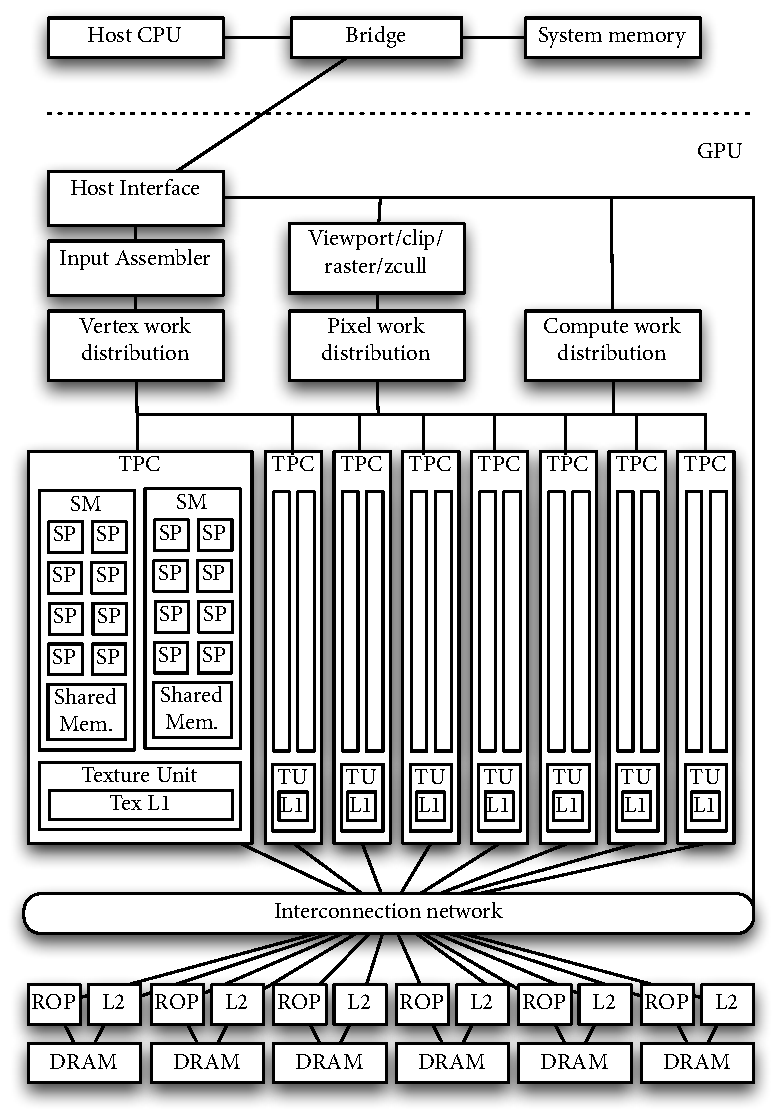
\includegraphics[width=\textwidth]{gfx/tesla_architecture} 
\caption{Tesla Architecture} 
\label{fig:tesla_architecture} 
\end{figure} 

The \autoref{fig:tesla_architecture} shows the Tesla architectures. As mentioned
above the new \gls{GPU} architectures are a radical departure from traditional
\gls{GPU} design. The Tesla 8 Series has 16 multiprocessors. Each multiprocessor
is composed of 8 streaming processors, 128 processors in total. Each streaming
multiprocessor has 16 \gls{KB} of shared memory and a L1 cache attached and has access
to a texture unit. A streaming processor consists of a scalar \gls{ALU} and
performs floating point operations. 32 streaming processor build up a \gls{SIMD}
unit in NVIDIA terms called warp, in that one instruction is executed. The Tesla
C870 has 1.5 \gls{GB} \gls{GDDR3} graphics memory, 519 \glspl{GFLOP} of peak
performance and \unitfrac[77]{\gls{GB}}{s} peak memory bandwidth. Many massively
data-parallel algorithms can be run sufficiently on this specialized
architecture \citep{citeulike:3145468}. Programming for this architecture is
done with \gls{CUDA} the C language extension which will be covered in the next
section.

\paragraph{The Mainstream GPU} % (fold)
\textbf{welche karte habe ich zum teufel}
 The 8800 GTX has 768 MB of graphics memory, 620 GFlops
of peak performance and 86 GB/s peak memory bandwidth. 
% paragraph the_mainstream_gpu (end)
\label{par:the_mainstream_gpu}


% section the_tesla_architecture (end)


\section{Common Unified Device Architecture (CUDA)}% (fold)
\label{sub:common_unified_device_architecture_cuda_} 
In 2007, NVIDIA introduced an extended \gls{ANSI} C programming model and
software environment the compute unified device architecture. The reason why
\gls{CUDA} was born is that parallelism is increasing rapidly with Moore's law
\footnote{Processor count is doubling every 18 - 24 months} and the challenge is
to develop parallel application software that scales transparently with the
number of processor cores. The main goals when \gls{CUDA} was developed were
that it scales to hundreds of cores, thousands of parallel threads and it allows
heterogeneous computing (\gls{CPU} + \gls{GPU}). All this considerations led to
the result that \gls{CUDA} runs on any number of processors without recompiling
an the parallelism applies to both \glspl{CPU} and \glspl{GPU} 
\citep{citeulike:3839013}.

\Gls{CUDA} is C with minimal extensions and defines a programming and memory model.
There are three key abstractions in \gls{CUDA}, a hierarchy of thread groups, shared
memories and barrier synchronization \citep{citeulike:3325943} that are exposed
to the developer. \Gls{CUDA} uses extensive multithreading where threads express
fine-grained instruction, data and thread parallelism that are grouped into
thread blocks which express coarse grained data and task parallelism. The
developer has to rethink about his algorithms to be aggresively parallel.
The problem has to be split into indepedent coarse sub-problems and at finer
level into fine-grained sub-problems that can be solved cooperatively
\citep{citeulike:3325943}.

\Gls{CUDA} has been accepted be many developers which can be seen by the huge
amount of already developed software and contributions to the \gls{CUDA}
zone \footnote{http://www.nvidia.com/cuda}.

A brief look shows the \gls{CUDA} computing sweet 
spots\citep{citeulike:3839013}

\begin{itemize}
	\item High arithmetic intensity (Dense linera algebra, PDEs, n-body, 
			finite difference, ...) 
	\item High bandwidth (Sequencing (virus scanning, genomics), sorting, 			
			database, ...) 
	\item Visual computing: (Graphics, image processing, tomography, 
			machine vision, ... ) 
	\item Computational modeling, science, engineering, finance, ... 			
\end{itemize} 

This is just a small snapshot of algorithms that can be used with \gls{CUDA} on
\glspl{GPU}. For a more extensive list and speedups compared to high-end
\glspl{CPU} see the webpage of NVIDIA
\href{http://www.nvidia.com/cuda}{\gls{CUDA} zone}. 
% section_unified_device_architecture_cuda_ (end)

\section{CUDA Programming Model}% (fold)
\label{sub:cuda_programming_model} 
The \gls{CUDA} programming model exposes the graphics processor as a highly
multithreaded coprocessor. The \gls{GPU} is viewed as a compute device to the
host that has its own device memory and runs many threads in parallel.

Applications are accelerated by executing data parallel portions of the
algorithm on the \gls{GPU} as \emph{kernels} which run in parallel on many
threads. There are some major differences between \gls{CPU} and
\gls{GPU} threads. A \gls{GPU} needs thousands of threads for full efficiency
where \glspl{CPU} only need a few of them. \Gls{GPU} threads have a very little
creation overhead and are extremely lightweight compared to \gls{CPU} threads.

\paragraph{Thread Batching}% (fold)
\label{par:thread_batching} 
A kernel is executed as a grid of thread blocks where data memory space is
shared by all threads. A thread block is a batch of threads that can cooperate
with each other by synchronizing there execution\footnote{For hazard free shared
memory access} and efficiently share data through the low latency shared
memory. Two threads from two different blocks can cooperate with atomic 
functions through the global memory. The identification of a thread is 
accomplished through block and thread ids which are assigned to each thread at 
creation time. 
% paragraph thread_batching (end)

\paragraph{Block and Thread IDs}% (fold)
\label{par:block_and_thread_ids} 
Every thread and block has a unique id. As a result of this each thread can
decide whata data to work on. For every block there is a assigned id in \gls{1D}
or \gls{2D} layout. Thread ids can be accessed either with \gls{1D}, \gls{2D} or
\gls{3D} coordinates similar to multidimensional arrays. It simplifies memory
addressing when processing multidimensional data( e.g image processing, matrix
multiplication or solving partial differential equations on volumes). The data
can reside in several levels of the device memory. % paragraph
%block_and_thread_ids (end)

\paragraph{Device Memory Space}% (fold)
\label{par:device_memory_space} 
The memory space is a hierarchy of several memory types that can be accessed per
thread, block, grid and the host. The threads have access to all memory levels
beginning with the \gls{RW} registers, local, shared, global, \gls{RO}
texture and constant memory. The grids have only access to global, constant
and texture memory. Whereas the \gls{CPU} can \gls{RW} global, constant and texture
memories.

Global, constant and texture memory have long latency accesses. They reside
off-chip where registers local\footnote{Not true for older \glspl{GPU} chips
where local data is spilled out to global memory} and shared memory resides
on-chip. The global, constant and texture memory are mainly used for
communication of \gls{RW} data between host and device where the contents is
visible to all threads. As mentioned above texture and constant memory can be
written by the host where constants and data are initialized.
% paragraph device_memory_space (end)


\section{A Simple Example}% (fold)
\label{sub:a_simple_example} 
This simple example will show the structure of an \gls{CUDA} program. The executing
kernel will do some easy calculations on the data provided, load the data into
shared memory  and write back the results to the global memory. 

A \gls{CUDA} program has a specific structure where the major parts are
described in this paragraph. The first thing to do is to initialize the device
and some auxiliary variables. Listing \autoref{lst:init} shows the
initalization.

%
\begin{lstlisting}[caption=Hardware initalization, label=lst:init]
int main( int argc, char** argv) {
	CUT_DEVICE_INIT(argc, argv);

	uint32_t num_threads = 32;
	uint32_t mem_size = sizeof(float) * num_threads;				
                  ...
\end{lstlisting} 
%

Since the \gls{GPU} is attached to the \gls{PCIE} bus the host has no direct
access to the global, constant and texture memory and has to transfer the data
back and forth with the \gls{DMA} engine of the device. This is accomplished
through the \gls{CUDA} \gls{API} calls that initiate the transfer. Before any
transfer can be done one has to allocate memory on the host and on the device
for input and output data. This is shown in listing \autoref{lst:datatransfer}.


\begin{lstlisting}[caption=Data transfer of data, label=lst:datatransfer]
	// allocate host memory 
	float* h_idata = (float*) malloc(mem_size);
	// allocate device memory 
	float* d_idata; cudaMalloc((void**) &d_idata, mem_size);
	// allocate device memory for result
	float* d_odata; cudaMalloc((void**) &d_odata, mem_size);
	// allocate mem for the result on host side
	float* h_odata = (float*) malloc( mem_size);
	// copy host memory to device 
	cudaMemcpy(d_idata, h_idata, mem_size, cudaMemcpyHostToDevice);
\end{lstlisting} 


After setting up the input data the setup execution parameters are defined that
are used to startup the kernel. The \textit{grid(1, 1, 1)} statement defines
a multi-dimensional array of grids \textit{x=1, y=1, z=1} whereas the
\textit{threads(num\_threads, 1, 1)} defines a multi-dimensional array of
threads \textit{x=num\_threads, y=1, z=1} which are actually \gls{1D} arrays.
\autoref{lst:execution} shows the call of the kernel with its input and
output data.


\begin{lstlisting}[caption=Execution of the Kernel, label=lst:execution]
	    // setup execution parameters
	    dim3  grid( 1, 1, 1);
	    dim3  threads(num_threads, 1, 1);

	    // execute the kernel
	    kernel<<< grid, threads, mem_size >>>(d_idata, d_odata);
\end{lstlisting} 

If everything went well the host can copy the data from device memory
to host memory and check, visualize or store the calculated values.
\autoref{lst:result} shows the last steps before exiting the program.

\begin{lstlisting}[caption=Retrieving of the Results, label=lst:result]
	    // check if kernel execution generated and error
	    CUT_CHECK_ERROR("Kernel execution failed");
 
	    // copy result from device to host
	    cudaMemcpy(h_odata, d_odata, sizeof( float) * num_threads, 
			       cudaMemcpyDeviceToHost);

	    // cleanup memory free(x), free(y), free(z) ...
		CUT_EXIT(argc, argv);
	} 
\end{lstlisting} 

The previous listings showed the host code and how to launch a kernel on the
device. The \autoref{lst:device} shows the device code portion. There are
several qualifiers that define which function is compiled for which processing
unit. The \textit{\_\_global\_\_} qualifier specifies that this function is run
on the device and hence compiled for the \gls{GPU} where the
\textit{\_\_host\_\_} qualifier specifies that this function is only run on the
host and not on the device. There are more function specifiers that can be
looked up in \citep{citeulike:3325943}.

For data there are as well qualifiers where one can specify where the data is
located, either in constant, global or shared memory. In \autoref{lst:device}
the \textit{\_\_shared\_\_} qualifier is used. The device will use the shared
memory to preload the data for faster access.


\begin{lstlisting}[caption=CUDA device code, label=lst:device]
	#include <stdio.h>

	#define SDATA(index) CUT_BANK_CHECKER(sdata, index)
	// Simple test kernel for device functionality
	__global__ void kernel( float* g_idata, float* g_odata) 
	{
	  // shared memory
	  // the size is determined by the host application
	  extern  __shared__  float sdata[];

	  // access thread id
	  const unsigned int tid = threadIdx.x;
	  // access number of threads in this block
	  const unsigned int num_threads = blockDim.x;

	  // read in input data from global memory
	  // use the bank checker macro to check for bank conflicts during host
	  // emulation
	  SDATA(tid) = g_idata[tid];
	  __syncthreads();

	  // perform some computations
	  SDATA(tid) = (float) num_threads * SDATA( tid);
	  __syncthreads();

	  // write data to global memory
	  g_odata[tid] = SDATA(tid);
	} 
\end{lstlisting} 


After loading the data the kernel just multiplies the thread-id with the number
of threads and saves the result back to global memory where the host can pick up
the result.
% section a_simple_example (end)
% section cuda_programming_model (end)
% section background_to_the_project (end)

\section{Porting Strategies for GPUs}.% (fold)
\label{sec:porting_strategies_for_gpu} 

\myChapter{Feasibility Study}
\label{chap:feas}
There are several myths about \gls{GPGPU} which will be examined and solved 
with a feasibility study. Listed below some myths in no particular order.
\begin{enumerate}
	\item \gls{GPU} programs are written with a graphics api and layered on top 
		of graphics
	\label{enum:api}
	\item \glspl{GPU} can only do a gather and no scatter memory access
	\label{enum:gather}
	\item \glspl{GPU} are power-inefficient
	\label{enum:ineff}
	\item \glspl{GPU} don't do real floating point math
	\label{enum:float}
	\item \glspl{GPU} in average one can only exploit about 10\% of the peak 
		performance for general purpose computing
	\label{enum:exploit}
	\item \glspl{GPU} are very wide \gls{SIMD} machines on which branching is 	  
		impossible, with 4-wide vector registers
 	\label{enum:simd}
\end{enumerate}

The most interesting myth here is that in average one can only exploit about
10\% of the peak performance for general purpose computing, which in turn would 
lead to that \glspl{GPU} are power-inefficient in average. Another thing to 
keep an eye on is the statement that \glspl{GPU} do not do real floating point
math which would exclude many communities (\gls{HPC}, Physics, Astronomy, ..)
\graffito{Many \gls{HPC}, Physics, Astronomy,... benchmarks and algorithms rely 
on floating point math} from spending time in doing \gls{GPGPU}. 

Therefore the first step before choosing an algorithm or put further energy into
research of \glspl{GPU} is to make a feasibility study. The study will examine
the myths and show solutions to the problems respectively statements.
Furthermore it will show whether the technology, software eco system exists for
building applications on \glspl{GPU} and how difficult it will be to build.

By the means of a ray tracer the study will show which steps have to be 
undertaken to gain high performance with an parallel algorithm and show which 
architectural points have to be considered when designing an application.

\section{An Overview of Ray Tracing}
Ray tracing is a technique for realistic image synthesis. Ray tracing as the
name says traces light rays generated from an imaginary camera to their points
of origin. Ray tracing is based upon a physical, mathematical model behind
light, which facilitates to render photo realistic images. 

Ray tracing can be seen as an extension to ray casting. Therefore its easier to
understand ray tracing if the base concept of ray casting are understood. The
next section will introduce ray casting \footnote{For an in depth description of
ray tracing on a parallel machine see \cauthor{citeulike:80546}
\citep{citeulike:80546}}.

\section{Ray Casting}
Ray casting was first introduced by \cauthor{Appel68} \citep{Appel68} he
developed some techniques for a shading machine for rendering of solids.

First of all it is important to understand the concept of rays. A ray is the
path of a particle of light (photon) extending from the eye into the
scene \cite{Glassner289}. The path is a thin, straight line used to model a beam
of light. Each ray can be seen as a \textit{feeler}\graffito{The ray scans or 
rasters the scene that is why a ray is often called a feeler} that reaches the 
scene and finds out which objects are visible and what color the object has at a 
specific point. Rays are the fundamental element of any ray tracer.

The representation of light on the screen is organized in so called pixels.
A pixel is a point sample not a little geometric square. This misconception
is widespread and it is an issue that strikes right at the root of correct
image computing and the ability to correctly integrate the discrete and the
continuous \cite{AlvyRaySmith95}.

The color of a given pixel is the color of the light that passes from the
object, through the associated pixel into the eye \cite{Hearn94}.

For each pixel on the screen a ray is cast from the eye through the pixel into
the virtual world. Then for each object it is checked if the ray intersects any
of them. If there are several objects in a scene intersected by the ray the
shortest distance to the intersection point is the one that is visible to the
eye. All other intersection are behind the nearest object and not visible
respectively occluded by the visible object. The color at that point is the
accumulated contribution of intensities radiated from all light sources. This
color is given to the pixel through which the ray passed. Ray casting does not
consider light reflected or transmitted by other objects in contrast to ray
tracing.

Ray casters and ray tracers spent most of their time calculating intersections
of rays with different objects. \cauthor{Whitted80} \citep{Whitted80} estimates
that anywhere from 75 percent to over 95 percent of rendering time is spent in
intersection tests. For example an image with 640 pixel width and 480 pixels
height, for a total of 307200 pixels, with a medium complex scene with 100
objects results in 30.720.000 intersection tests. There are well documented ray
tracing accelerating techniques not only to decrease the number of intersection
tests per ray but also to decrease the number of rays.

In the study the standard ray casting algorithm will be used only, which means
that every ray will be intersected with every object to have a high arithmetic
density and not to be limited by the memory bandwidth.

Further experiments to extend the basic ray casting algorithm to ray tracing 
will be discarded this will only add more complexity to the algorithm and will
not help in solving the essential problems. 

\section{Performance tuning} % (fold)
\label{sec:performance_tuning}

After the initial port of the ray tracer to \gls{CUDA}, the first goal was to 
make it run on the \gls{GPU}, it was time to fine tune the run configuration. 
For any \gls{CUDA} application it is crucial to take a look at register, shared 
memory and local memory usage. The performance of the application is depend on
how good/bad the existing resources are exploited.

The examination of the ray traced showed that the initial port used 48
registers, 28 bytes shared memory and 96 byte constant memory per thread. As
shown in \textbf{REF. to CUDA Application Stuff} the number of launched threads,
blocks and grids is dependent on the three factors mentioned above.

Each \gls{SM} has 8192 registers which means we could have 8192/48 = 170 threads
to fully exploit the resources 8 blocks should be launched so 170/8 = 21 threads per block which is by far too low. It is easily spotted that the application is
limited by registers / \gls{SM}. These calculations can easily be done with the \emph{CUDA occupancy calculator} supplied with the SDK. 

After fiddling around with compiler switches especially \emph{-maxrregcount=x}
the application used only 14 register which meant we could have a blocksize of
8, 8x8 = 64 threads per block \graffito{It is always good to have a thread count
which is a multiple of 32. A warp consits of 32 threads and the scheduler can
easier schedule the threads}. When reducing the amount of registers used, one
has to consider that registers which are additionally needed are allocated from
the local memory rather than the register file. Local memory is located in the
global memory which has a high latency (200-400 cycles) and registers often
referenced have a big impact on performance. The application can become memory
bound.

The Table \ref{tab:runconfig} shows the run configuration used for the sample runs. 

\begin{table}[ht]
    \myfloatalign
  \begin{tabularx}{\textwidth}{ccccc} \toprule
	\multicolumn{5}{c}{\spacedlowsmallcaps{Run Configuration}} \\ \midrule
	blockSize.x & blockSize.y & gridSize.x & gridSize.y & Regs. per Thread\\ 
  	8 & 8 & 96 & 96 & 14\\
    \bottomrule
  \end{tabularx}
  \caption[Run configuration]{Run configuration.}
  \label{tab:runconfig}
\end{table}

To summarize just by compiling the application and fiddling with the run
parameters one can achieve, in this case, a speedup of about 8 times. See Table
\ref{tab:comp} for several runs varying object count and image size.

\begin{table}[ht]
   \myfloatalign
  \begin{tabularx}{\textwidth}{ccccc} \toprule
    \tableheadline{Image} & 
	\tableheadline{Objects} & 
	\tableheadline{CPU Gflops} &
	\tableheadline{GPU Gflops} &
	\tableheadline{Speedup}\\ \midrule
    768 & 338 &  0.37 & 3.17 & 8.54 \\
 	768 & 450 &  0.37 & 3.22 & 8.6\\
 	768 & 840 &  0.37 & 3.23 & 8.74\\ 
 	512 & 338 &  0.37 & 3.19 & 8.53\\
 	512 & 450 &  0.37 & 3.18 & 8.5\\
 	512 & 840 &  0.37 & 3.18 & 8.64\\ 
 	256 & 338 &  0.37 & 3.03 & 8.09\\
 	256 & 450 &  0.37 & 3.03 & 8.44\\
 	256 & 840 &  0.37 & 2.95 & 7.96\\
    \bottomrule
  \end{tabularx}
  \caption[Comparison between CPU and GPU]{Comparison between CPU and GPU.}
  \label{tab:comp}
\end{table}

As it can be seen in Table \ref{tab:comp} the application runs 8 times faster but when looking at the \glspl{GFLOP} values there are far beyond that what a \gls{GPU} could achieve\footnote{The used \gls{GPU} is a G90 chip with peak 620 \glspl{GFLOP}}. The application is only using 0.5\% of the peak performance!\graffito{All performance values are gathered with the NVIDIA Performance Profiler availabe as well with the \gls{SDK}}  


The reasons for this uneffective usage of processing power can be seen in Table \ref{tab:localmem} and Table \ref{tab:globalmem}. The application is heavily memory bound. The consequence of reducing the register usage is heavy access to local memory, e.g. there are over 328000000 stores issued to the memory. Furthermore the code is using many branches which actually reflected by the value 22578032. 

\begin{table}[ht]
    \myfloatalign
  \begin{tabularx}{\textwidth}{cccc} \toprule
	\multicolumn{2}{c}{\spacedlowsmallcaps{Local Memory}} &
	\multicolumn{2}{c}{\spacedlowsmallcaps{Branches}} \\ \midrule
    Load & Store & Sum & Divergent\\
	63294179 & 328180560 & 22578032 & 26834\\
    \bottomrule
  \end{tabularx}
  \caption[Local memory and branches]{Local memory and branches.}
  \label{tab:localmem}
\end{table}

Another point is the access to global memory. The \gls{GPU} is able to do coalesced reads and writes when possible otherwise the access is serialized. 
The application was not ported with coalesced memory reads and writes in mind and hence the application is loading almost everything incoherent. See Table \ref{tab:globalmem} for the values. 

\begin{table}[ht]
    \myfloatalign
  \begin{tabularx}{\textwidth}{cccc} \toprule
	\multicolumn{4}{c}{\spacedlowsmallcaps{Global Memory}} \\ \midrule
    Load Incoherent & Load Coherent & Store Incoherent & Store Coherent \\
	1115657863 & 67961 & 2506752 & 0 \\
    \bottomrule
  \end{tabularx}
  \caption[Global memory loads and stores]{Global memory loads and stores.}
  \label{tab:globalmem}
\end{table}

The ray tracer could be extended or optimized in many ways but it will be leaved as is. The main point of the feasibility study was to get a \emph{feeling} for developing on \glspl{GPU} and to spot major drawbacks and obstacles. Keeping the lessons learned here in mind the development of the main application will be easier. The following section will demystify some but not all myths stated in the beginning.
% section performance_tuning (end)

\section{Demystifing the Myths} % (fold)
\label{sec:demystifing_the_myths}
There were several myths about \gls{GPGPU} see \ref{chap:feas} that are simply wrong or need to be proven. Beginning with \ref{enum:api} this statement is 
simply wrong. Using \gls{CUDA} or the ATI \gls{SDK} \emph{Close To Metal}
no developer is anymore forced to use graphics \glspl{API}. Furthermore the abandoned graphics \gls{API} for \glspl{GPGPU} makes it possible to gather and scatter to the memory, which resolves myth \ref{enum:gather}. 

The \glspl{GPU} are able to do real floating point math. The myth \ref{enum:float} comes from a time where floats were only 16 or 24 bit and had no support for \emph{NaN}, \emph{Rounding to zero} and so on. The situation changed completely with the recent development and the switch to the \emph{Unified Device Architecture} where \gls{SIMD} processing was discarded in 
favour of more single independent threads. 

The last to myths \ref{enum:ineff} and \ref{enum:exploit} are hard to demystify.
If one has a algorithm which fits excellently to the \gls{GPU} the full power of
the \gls{GPU} can be exploited and hence it is power efficient. It depends
heavily on the algorithm. The feasibility study has shown that one can achieve
easily a speedup but considering the inefficient use of the ressources and the
power dissipation it could be a slow down investing so much power for so little
return.

% section demystifing_the_myths (end)








%*******************************************************************************
\chapter{Mean Shift}\label{ch:mean_shift}
%*******************************************************************************
In low level computer vision tasks like segmentation, edge detection or smoothing
the analysis of data is often not done on the original images. Features like 
colors are rather projected into a feature space where they can be more easily
analyzed. The analysis of the feature space can find interesting attributes of 
the image like edges or segments.

The feature space has to be smoothed before analysis. Feature spaces originate
from real images therefore they are composed of several components from
different distributions. The basic approach of a mixture model, a mixture model
is a probabilistic model for density estimation using a mixture distribution, is
not efficient enough to estimate the density satisfactorily of such complex,
arbitrarily comprised densities. The discontinuity preserving smoothing is therefore
accomplished with kernel based density estimators. Kernel based density estimators
are making no assumptions about densities and hence can be estimate aribtrary 
densities.

The maxima of a feature space correspond to the searched components like edges
of an image. Gradient based methods of feature space analysis are using gradients
of the probability density function to find the maxima. Such methods are complex
because they need among other things a estimation of the probability density.

Mean shift is an alternative to the gradient based methods as it is easier to 
calculate then to estimate the probability density and then to calculate the 
gradient. The mean shift vector points to the same direction as the gradient of
gradient based methods. Furthermore the mean shift vector has a adaptive size and
is non parametric. There is no need to supply a step size compared to the other
methods. Mean shift a robust approach toward feature space analysiswas
originally introduced by \citeauthor{citeulike:462300} \citep{citeulike:462300}.

\section{Density Estimation} % (fold)
\label{sec:density_estimation}
In probability and statistics it is known that for different tasks there exist 
more or less suitable features. In 
\citep{citeulike:167581} \citeauthor{citeulike:167581}  are giving an example of 
a classification of two different fish types. 


\section{Kernel Density Estimation} % (fold)
\label{sec:kernel_density_estimation}
Kernel density estimation is a method to estimate an unkown density
distribution with finite observations of a point in the sample space. 
The result of such a procedure is a probability density function that describes 
the density of probability at each point in the sample space. To estimate the 
density of a point $x = { x_1, ... , x_d, ... , x_D} \in \mathbb{R}^D$ in a 
$D$ dimensionl feature space, $N$ observations $x_1^N$ with
 $x_N \in \mathbb{R}^D$ within a search window that is centered around point $x$
have to be observed. The search window with radius $h$ is the bandwidth of the
used kernel. The density of probability in point $x$ is the mean of density of
{\color{iRed}probabilities falling into the search window.}

The effect of different bandwith parameters $h$ (search window radius) is shown in 
\autoref{fig:window_radius}. The example shows a kernel density estimation with
five observations $x = 4, 1, -1, -3, -3.5$ and a normal kernel. The total density
estimation is the sum of each kernel at a observation, here shown for three 
bandwidths. With bigger bandwidth $h$ the density estimation becomes smoother.  

\begin{figure}[ht]
\centering
%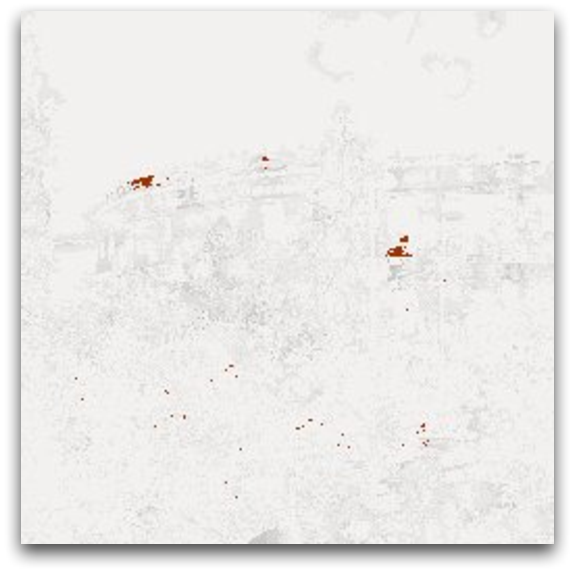
\includegraphics[width=0.6\textwidth]{gfx/itr_limitcycle0.pdf}
\caption{Effect of bandwidth selection}
\label{fig:window_radius}
\end{figure}


Kernel density estimation is a non parametric method, although some parameters
exists like the search window radius. Non parametric methods are making no 
assumptions about the density of probabilities. The strenght of such methods is
that they are not limited to just on probability but can deal with arbitrary
coupled/joined probabilities. With an unfinite number of observations the non
parametric methods can reconstruct the density of the original
probabilities.

To derive the kernel density estimator in point $x \in \mathbb{R}^D$ first of
all some definitions have to be made. Let $x$ be a random variable and $N$
observations $x_1^N$ with $x_n \in \mathbb{R}^D$ given. The kernel density
estimator $\hat(f)(x)$ in a point $x \in \mathbb{R}^D$, with a kernel $K(x)$ and a
$DxD$ bandwith matrix $\mathbf{H}$ is 
\begin{equation}\label{eq:kernel0}
	\hat{f}(x) = \frac{1}{N} \sum_{n = 1}^N K_{\mathbf{H}}\left( x-x_n \right)
\end{equation} 
where
\begin{equation}\label{eq:kernel1}
	K_{\mathbf{H}}(x) = \frac{1}{\sqrt{|\mathbf{H}|}}K \left( \frac{x - x_n}{h} \right)
\end{equation} 

Since a full parametrized matrix $\mathbf{H}$ would lead to very complex estimates
only a single bandwidth parameter, the window radius will be regarded. With the
simplification $\mathbf{H} = h^2 \mathbf{I}$ the \autoref{eq:kernel0} can be 
written as
\begin{equation}\label{eq:kernel2}
	\hat{f}(x) = \frac{1}{Nh^D}\sum_{n=1}^N K\left( \frac{x - x_i}{h} \right).
\end{equation}

The kernel density estimator is valid for several kernels and successive
considerations will deal with several kernel the \autoref{eq:kernel2} will be
formated into a more generic form. For this transformation the definition of a
kernel and profile of the kernel is needed. The following definition of a kernel
and its profile is from \citeauthor{citeulike:2522867}
\citep{citeulike:2522867}. The norm $\lVert x \rVert$ of $x$ is a non negative number 
so that $\lVert x \rVert^2 = \sum_{d = 1}^D|x_d|^2$.
A $K:\mathbb{R}^D \rightarrow \mathbb{R}$ is
a known as a kernel, when there is a function $k:[0, \infty] \rightarrow \mathbb{R}$ the profile
of the kernel, so that
\begin{equation}\label{eq:kernel3}
	K(x)=c_{k,d}k(\lVert x \rVert^2)
\end{equation}
where $K$ is radial symmetric, $k$ is non negativ {\color{iRed} nicht zunehmend
und stückweise stetig ist} with $\int_0^{\infty} k(r) dr < \infty$. $c_{k,D}$ is
a positive normalization constant so that $K(x)$ integrates to $1$. 

Now the kernel density estimator from \autoref{eq:kernel2} can be transformed into
a new equation. The two indices $K$ and $h$ are representing which kernel and 
which radius are used for the density estimator. With the profile notation $k$, where
\autoref{eq:kernel2} is inserted into \autoref{eq:kernel1}, the \autoref{eq:kernel2}
is transformed to
\begin{equation}\label{eq:kernel4}
	\hat{f}_{h,K}(x) = \frac{c_{k,D}}{Nh^d}\sum_{n = 1}^N k(\lVert \frac{x-x_n}{h} \rVert^2)
\end{equation}



\section{Kernel Properties} % (fold)
\label{sec:kernel_properties}








\section{OLD STUFF} % (fold)
\label{sec:old_stuff}

We consider the kernel
estimator in
$\mathbb{R}^1$. Let $X$ be a random variable. Let $X_i$ where $i=1,2,\ldots,n$ be
% estimate	= schätzen
% density	= dichte
$n$ observations of $X$. We want to estimate the density  of $X$. Let $f$ be the
density of $X$, and $\hat{f}$ an estimator of $f$. A \emph{bin} is an interval
$[a,b)$. $b-a$ is called the width of bin $[a,b)$. Let $O=(0,0)$ be the origin, 
and $[mh, (m+1)h)$ are some bins of constant width $h$, for integers $m$. The
histogram is defined as follows,
\begin{equation}\label{eq:histogram}
	\hat{f}(x)=\frac{1}{nh} \times n_i
\end{equation}
where $n_i$ is the number of $X_i s$ in the same bin as $x$.

The histogram is the oldest and most frequently used density estimator. But it 
comes with drawbacks. For example, the histogram is not continuous (thus, it 
does not have derivatives); it depends on the position of the origin; and a 
% multivariate	= involving two or more variable quantities.
technique based on histograms is difficuld to generalize to the multivariate 
case. The \emph{native estimator} is a generalization of the histogram 
technique. Since $f$ is the density function of $X$, we have
\begin{equation}\label{eq:naive_estimator}
	f(x) = \lim\limits_{h \rightarrow 0} \frac{1}{2h} \times P(X \in (x-h,x+h))
\end{equation}

where $P(X \in (x-h,x+h))$ is the probability of $X$ falling into $(x-h,x+h)$.
The naive estimator is defined as follows:
\begin{equation}\label{eq:naive_estimator2}
	\hat{f}(x) = \frac{1}{2nh} \times n_i^{\prime}
\end{equation}
where $n_i^{\prime}$ is the number of $X_i s$ falling into $(x-h,x+h)$. 

If $x$ is the center of a bin of the current histogram, then Equation 
\eqref{naive_estimator2} will be equal to Equation \eqref{naive_estimator}. 
Therefore, the naive estimator is a generalization of the histogram technique.
Equation \eqref{naive_estimator2} can also be written as
\begin{equation}\label{eq:naive_estimator3}
	\hat{f}(x) = \frac{1}{nh}\sum_{i=1}^n w\left( \frac{x - X_i}{h} \right)
\end{equation}
where $w$ is defined as 
\begin{equation}\label{naive_estimator3}
	w(x) = \begin{cases}
				1/2 & \text{if } x \in (-1,1) \\
				0 & \text{otherwise }
		\end{cases}
\end{equation}

The naive estimator "inherits" some drawbacks of the histogram technique.
For example, it is not continuous: it "jumps" at points $X_i \pm h$ and has a 
zero derivative for each $x \neq X_i \pm h$.

The naive estimator can be further generalized to a \emph{kernel estimator}. 
Replace function $w$ in Equation \eqref{eq:naive_estimator3} by a function $K$;
we obtain
\begin{equation}\label{eq:kernel_estimator}
	\hat{f}(x) = \frac{1}{nh} \sum_{i=1}^n K\left( \frac{x - X_i}{h} \right)
\end{equation}

where $K$ is requested to satisfy the following condition

\begin{equation}\label{eq:kernel_condition}
	\int_{-\infty}^{\infty} K(x)dx = 1
\end{equation}
because $K(x)$ is a density function.

If $K$ has a derivative, for each $x \in (-\infty, +\infty)$, then by Equation
\eqref{eq:kernel_estimator} so does the kernel estimator. For example, let $K$
be the normal density function, to construct a kernel estimator which has a 
derivative for each $x \in (-\infty, +\infty)$. In Equation \eqref{eq:kernel_estimator}, $h$ is called the \emph{window width (smoothing parameter, or bandwidth); K is called the kernel} function. 
Analogously, we can define the kernel estimator in $\mathbb{R}^d$:
\begin{equation}\label{eq:kernel_estimator_rd}
	\hat{f}(x) = \frac{1}{nh^d} \sum_{i_1}^n K\left( \frac{x-X_i}{h} \right)
\end{equation} 
where $K$ satisfies the following condition
\begin{equation}\label{eq:kernel_rd_condition}
	\int_{R^d} K(x)dx = 1
\end{equation}

In summary, the kernel estimator is an estimator of the density function of a 
random variable, represented by a sum of some simple kernel functions such that
the estimator has "good" mathematical properties such as being differentiable,
symmetric, and so forth.
% subsubsection the_kernel_density_estimator (end)



\subsubsection{The Mean Shift Procedure} % (fold)
\label{ssub:the_mean_shift_procedure}
This subsection explains the principle of \textbf{adaptive?!?} mean shift-based
clustering, meaning that the data points always move to local density maxima.

We review some results of [8]. Let $k(x)$ be a symmetric univariate kernel 
function, where $x \in (-\infty, +\infty)$. We can construct a $dD$ kernel 
function from $k(x)$ as follows:
\begin{equation}\label{eq:dd_kernel}
	K(x)=c_{k,d}k(\lVert x \rVert^2)
\end{equation}
where
\begin{equation}\label{eq:kernel_constant}
	c_{k,d} = \frac{\int_{R^d} K(x) dx} {\int_{R^d} k(\lVert x \rVert^2) dx} = \frac{1}{\int_{R^d} k(\lVert x \rVert^2) dx} > 0
\end{equation}
Function $k(x)$, where $x \in [0, +\infty)$, is called the \emph{profile} of the
kernel $K(x)$. 

By Equation \eqref{eq:dd_kernel}, the kernel density estimator [see Equation \eqref{eq:kernel_estimator_rd}] can be rewritten as follows:

\begin{equation}\label{eq:label}
	\hat{f}_{h,K}(x) = \frac{c_{k,d}}{nh^d}\sum_{i_=1}^n k(\lVert \frac{x-X_i}{h} \rVert^2)
\end{equation}

Suppose that $k(x)$ is differentiable in $[0, +\infty)$, except for a finite 
number of points.
\begin{equation*}\label{eq:shadow_kernel}
	g(x) = -k\prime(x)
\end{equation*}

where $x\in [0, +\infty)$, except for a finite number of points. Construct a 
kernel function from $g(x)$ as follows:
\begin{equation*}\label{eq:shadow_kernel1}
	G(x) = c_{g,d}g(\lVert x \rVert^2)
\end{equation*}

where
\begin{equation}\label{eq:shadow_constant}
	c_{g,d} = \frac{\int_{R^d} G(x) dx} {\int_{R^d} g(\lVert x \rVert^2) dx} = \frac{1}{\int_{R^d} g(\lVert x \rVert^2) dx} > 0
\end{equation}

Denote the gradient of the density estimator of $\hat{f}_{h,K}(x) \text{by} \nabla \hat{f}_{h,K}(x)$. Furthermore (see [8] for the details), let 
\begin{equation}\label{eq:mean_shift0}
	m_{h,G}(x) = \frac{1}{2}h^2 \frac{c_{g,d}}{c_{k,d}} \times \frac{\nabla \hat{f}_{h,K}(x)}{cd_{h,G}(x)}
\end{equation}
where
\begin{equation}\label{eq:mean_shift1}
	m_{h,G}(x) = \frac{\sum_{i=1}^n x_i g\left(\left\lVert \frac{x - x_i}{h} \right\rVert^2\right)}{\sum_{i=1}^n g\left(\left\lVert \frac{x - x_i}{h} \right\rVert^2\right)} -x
\end{equation}

Equation \eqref{eq:mean_shift1} is the difference between the weighted mean and
$x$, known as \emph{mean shift vector}. Since the gradient of the density estimator always points towards that direction in which the density rises most quickliy, by Equation \eqref{eq:mean_shift1}, the mean shift vector always points towards the direction in which the density rises most quickly. This is the main principle of the mean shift based clustering. 
% subsubsection the_mean_shift_procedure (end)


% section theory (end)

The mean shift algorithm is a nonparametric clustering technique which does not
require prior knowledge of the number of clusters, and does not constrain the
shape of the clusters. 

Given $n$ data points $x_i, i = 1, ... , n$ on a
$d$-dimensional space $R^d$, the multivariate kernel density estimate obtained
with kernel $K(x)$ and window radius $h$ is
\begin{equation}\label{density_estimator}
	f(x)=\frac{1}{nh^d}\sum_{i=1}^n K(\frac{x-x_i}{h}).
\end{equation}

For radially symmetric kernels, it suffices to define the profile of the kernel
$k(x)$ satisfying
\begin{equation}
	K(x)=c_{k,d}k(\lVert x \rVert^2)
\end{equation}
where $c_{k,d}$ is a normalization constant which assures $K(x)$ integrates to 
$1$. The modes of the density function are located at the zeros of the gradient
function  $\nabla f(x) = 0$.

The gradient of the density estimator \eqref{density_estimator} is 
\begin{equation}
	\begin{split}
		\nabla f(x) & = \frac{2c_{k,d}}{nh^{d+2}}\sum_{i=1}^n \left(x_i -
        x\right)g\left(\left\lVert \frac{x - x_i}{h} \right\rVert^2\right) \\ &
        = \frac{2c_{k,d}}{nh^{d+2}} \left[ \sum_{i=1}^n g\left(\left\lVert
        \frac{x - x_i}{h} \right\rVert^2\right) \right] \left[
        \frac{\sum_{i=1}^n x_i g\left(\left\lVert \frac{x - x_i}{h}
        \right\rVert^2\right)}{\sum_{i=1}^n g\left(\left\lVert \frac{x - x_i}{h}
        \right\rVert^2\right)} -x \right].
	\end{split}
\end{equation}
where $g(s) = -k'(s)$. The first term is proportional to the density estimate at
$x$ computed with kernel $G(x) = c_{g,d}g(\lvert x \rvert^2)$ and the second 
term
\begin{equation}
	m_h(x) = \frac{\sum_{i=1}^n x_i g\left(\left\lVert \frac{x - x_i}{h} \right\rVert^2\right)}{\sum_{i=1}^n g\left(\left\lVert \frac{x - x_i}{h} \right\rVert^2\right)} -x
\end{equation}
is the \emph{mean shift}. The mean shift vector always points towards the direction of the maximum increase in the density. The mean shift procedure, obtained by successive
\begin{itemize}
	\item computation of the mean shift vector $m_h(x^t)$,
	\item translation of the window $x^{t+1} = x^t + m_h(x^t)$
\end{itemize}
is guaranteed to converge to a point where the gradient of density function is
zero. Mean shift mode finding process is illustrated in \autoref{mean_shift0}.

The mean shift clustering algorithm is a practical application of the mode
finding procedure:
\begin{itemize}
	\item starting on the data points, run mean shift procedure to find the 
	stationary points of the density function,
	\item prune these points by retaining only the local maxima.
\end{itemize}

The set of all locations that converge to the same mode defines the \emph{basin of attraction} of that mode. The points which are in the same basin of 
attraction is associated with the same cluster. \autoref{mean_shift1} shows two examples of mean shift clustering on three dimensional data.






\chapter{Mean Shift Algorithm Analysis} % (fold)
\label{ch:algorithm_analysis}
Before any porting can be started the developer has to find out if
there are multiple activities or tasks which can run simultaneously
which expose exploitable concurrency. The developer has to find
concurrency either by decomposing the data or tasks. By this
decomposition one wants to solve bigger problems in less time as
several processing units can solve different parts of the problem.

But before any analysis is started one has to know if the problem is
large enough and if the resulting speedup justifies all the effort
that is expended on making a parallel version out of it. In case of
mean shift which is used for several things like filtering,
segmentation, pattern recognition and real time tracking one can
deduce that for bigger images or many images the computation time
climbs fast as the size or the number of images rises. To have a clue
how the mean shift algorithm behaves with big pictures several run
times where recorded.  For the analysis of the mean shift algorithm a
ready to use \gls{EDISON} was used that was profiled and modified and
parallelized for the purpose of this thesis.

The \gls{EDISON}
\footnote{http://www.caip.rutgers.edu/riul/research/code/EDISON/index.html}
system which was developed by the authors
\citeauthor{citeulike:462300} of \citep{citeulike:462300} offers
functionality to filter, segment and detect edges in images.
 
The \autoref{fig:cpu_run_time} shows results of \gls{CPU} run times of
the \gls{EDISON} application dependant on image size. The vertical
axis shows the run time in seconds and the horizontal axis shows the
side length in pixels of the quadratic \autoref{fig:orig0}.
\begin{figure}[ht]
  \centering
  \begin{tikzpicture}
    \begin{axis}[
      % smooth,
      % stack plots=y,
     % area style,
      ybar, bar width=8pt,
      width=\textwidth,
      height=5cm,
      xtick={128,384,...,2688},
      axis x line=bottom,
      axis y line=left,
      xmin=128, xmax=2816, 
      % ymin=0, 
			ymax=7000,
      xlabel=Image size, ylabel={Seconds [s]}, 
			%enlargelimits=0.03,
      %ymajorgrids
 			]
      \addplot[color=pl0,fill=pf0]
      table[x=PIX] {Plots/single.gpu.data}%
      \closedcycle;
    \end{axis}
  \end{tikzpicture}%
  \caption{CPU run time depending on the image size}\label{fig:cpu_run_time}%
\end{figure}
Considering the numbers in the result one can see that the run times
grow linear to the image sizes. The mean shift algorithm has linear
complexity, hence its complexity can be written as $O(n)$. Doubling
the side length of the quadratic picture the run time increase by a
factor of 4. See e.g.  the run times for side length: (l=256, t=9) and
(l=512, t=36).
    
But this is obvious, as stated in \autoref{ch:mean_shift} for each
pixel of the image the mean shift vector has to be calculated, and if
one increases the number of pixels by a number $n$ we have to deal
with $n$ times longer run time. Such consideration have to be done in
the run-up to have a clue to which point the algorithm can be
accelerated. The problem has to be well understood.

The next important step is to find parts which can be offloaded to an
accelerator as the \gls{GPU}. A first good point for such parts is to
make a profiling of the application to find out the most
computationally intensive parts. It makes no sense to parallelize
functions which contribute only 1\% to the run time.
    
\section{Profiling the Original Code} % (fold)
\label{sec:run_time_analysis_of_the_original_code}
A good start point is to take a profiler und generate a profile of the
functions, recording their run time and call history. In this case a
statistical profiler is used which operates by sampling. The samples
are taken from the hardware performance counters which every modern
\gls{CPU} has builtin.
OProfile\footnote{http://oprofile.sourceforge.net/news/} a system wide
profiler for Linux was used to examine the run time of the
\gls{EDISON} program. The \autoref{tab:comped} shows the run time
analysis of \gls{EDISON}.

\begin{table}[ht]
  \centering
  \pgfkeys{/pgf/number format/.cd,fixed zerofill,precision=2}
  \pgfplotstabletypeset[
  % column type=r,
  every row no 5/.style={
    before row={\rowcolor{pf0}}
  },
  columns/Self/.style={column type=r, column name={Self (\%)}},
  columns/Total/.style={column type=r, column name={Total (\%)}},
  columns/Symbol/.style={string type, column type=l, column name={Symbol}}
  ]{Tables/run.time.edison.data}
  \caption[EDISON run time profile]{ \gls{EDISON} run time analysis}
  \label{tab:comped}
\end{table}

Before taking a closer look at the table, the columns have to be
explained. The column \emph{Total} shows how long the function plus
their child function were executing. Whereas the column \emph{Self}
shows how long the function spent executing itself without the
execution time of their child functions. The column \emph{Symbol}
shows the function that was executed.

Now having a look at the table there is one function which is
executing 98.2\% of the run time, the function
\emph{uniformLSearch(double*, double*)}. In this function the
algorithm tries to find feature points that fall into the search
window with radius $h$ (see \autoref{sec:mean_shift}). This is the
starting point as it is the most computationally intensive and the
focus for parallelization. There is a way to calculate to which extent
the particular function can be parallelized and which speedup one can
expect. Speedup is the ratio of run time when executing a program on a
single processr to the run time when using $n$ processors. Given $T_1$
the run time of a program on a single processeor and $T_n$ the run
time of the same program on $n$ processors then
\begin{equation}\label{eq:speedup}
  S(n) = \frac{T_1}{T_n}
\end{equation}
is a measure for the speedup. One familiar law to calculate the how
much speedup can be obtained through paralellism is Amdahl's law.

\section{Amdahl's law}
\label{sec:amdahl_s_law}
Amdahl's law says supposing that 80\% of a computation can be
parallelized and 20\% can't, then even if the 80\% that is parallel
were run on an infinite number of processors the highest speedup that
one can achieve is 5. Generally speaking if a fraction $p$ of a
computation can be run in parallel and the rest must run serially,
Amdahl's law upper bounds the speedup by $1/(1-p)$.

The speedup of a application according to Amdahl is given by
\begin{equation}\label{eq:amdahl}
  S_{max}(n) = \frac{1}{(1-p) + \frac{p}{n}}
\end{equation} 
where $1$ is the execution unit time of the old computation, $(1-p)$
the inherently serial part and $p/n$ the parallel part divided by $n$
the number of processing units. When $n \rightarrow \infty$ then the
execution time approaches the time for executing the sequential
program fraction. So no matter how many processors one adds to the
system it will at least execute as long as the sequential program
fraction, which is an upper bound of speedup. A important addition is
that the sequential program fraction or serial processing percentage
is relative to the overall execution time using a single processor. It
is independent of the number $n$ of processors
\citeauthor{citeulike:3838998} \citep{citeulike:3838998}.

Assuming that the mean shift filtering can be parallelized with any number of
processing units one can calculate the maximum speedup achieveable according to
Amdahl. Taking the parallel processing percentage from \autoref{tab:comp} for
the filtering step:
\begin{equation*}\label{eq:parallel}
  p = 99,3\% = 0.993 
  p\end{equation*}
we get

\begin{equation*}\label{eq:am0}
  S_{max}(n) = \frac{1}{(1-0.993)} = \frac{1}{0.007} = 142.857	
\end{equation*}

Applying the calculation with $n = 128$, the used \gls{GPU} has 128
processors one can acheive a speedup of:
\begin{equation*}\label{eq:g92sp}
  S_{max}(128) = \frac{1}{(1-0.993) + \frac{0.993}{128}} = \frac{1}{0.007 + 0.0077578125} = 67.76
\end{equation*}
One can see that even for very small serial processing percentage the speedup is
not very high. Therefore \citeauthor{citeulike:3732921} proposed a alternative
formulation where the fractions are now dependent on $n$. He assumed that for
larger problem, the fraction of a program to parallelization increases. Thats
why Gustafson's law is often referred as a scaled speedup measure and Amdahl's
as a non scaled speedup measure. Given the serial $s'$ and paralllel time $p'$ a
single processor would require $s' + p' \times n$ time to finish the execution.
The speedup is then given by:
\begin{equation}\label{eq:gus}
  S_{max}(n) = \frac{s' + p' \times n}{s' + p'} = n + ( 1 - n ) \times s'
\end{equation}
Applying the calculation with $n = 128$, the used \gls{GPU} has 128 processors
one can acheive a speedup according to Gustafson of:
\begin{equation*}\label{eq:g92sp}
  S_{max}(128) = 128 + (1 - 128) \times 0.007 = 127.11
\end{equation*}

It looks like that Amdahl's \& Gustafson's law are in contradiction but looking
more precise on both definitions one can see that both laws employ different
definitions for the fraction of the serial and parallel exectuion times. Amdahl
uses non scaled percentage and Gustafson scaled percentage. Mathematicaly they
are equal just two different formulations. The scaled percentage can be
transformed to a non scaled perecentage where Gustafson's law gives the same
results as Amdahl's law \citep{citeulike:3838998}.

In summary one can expect more than a 100 fold speedup when parallelizing the
filter step of the mean shift algorithm. The next steps will focus on analyzing
how the mean shift filter can be decomposed to take advantage of multiple
processors.

\section{Data and Task Parallelism} % (fold)
\label{sec:data_and_task_parallelism}
There are two ways to decompose an algorithm to take advantage of parallelism.
The first way is to decompose the algorithm into several tasks that can run
independently. Each task is performing independently different calculation on
the data. This characteristic is known as task parallelism. To know if two task
can run independent one can take \citeauthor{citeulike:6113408} conditions and
evaluate them.

Let $P_i$ and $P_j$ be two tasks of a program $P$. For $P_i$ let $I_i$ be the
input and $O_i$ the output data and for $P_j$ let $I_j$ be the input and $O_j$
be the output data, then $P_i$ and $P_j$ are independent if they satisfy the
following conditions
\citep{citeulike:3838998}:
\begin{subequations}\label{eq:bern_cond}
  \begin{align}
    I_j \cap O_i & = \emptyset \label{eq:bern0}\\
    I_i \cap O_j & = \emptyset \label{eq:bern1}\\
    O_i \cap O_j & = \emptyset \label{eq:bern2}
  \end{align}
\end{subequations}
The first two formulations \autoref{eq:bern0} and \autoref{eq:bern1} are stating
that the input of one task has to be independent from the other task. Otherwise
one task would have to wait for the output of the other task to continue.
Furthermore not only the inputs vs. the outputs have to be independent but also
the outputs of each task have to be independent. If the above conditions cannot
be applied to a program $P$ than it is likewise that race conditions and poor
performance can arise through e.g. excessive synchronization overhead.


\subsection{Task Parallelism} % (fold)
\label{sub:task_parallelism}

Equipped with the knowledge how to identify independent parallel tasks, the mean
shift segmentation algorithm \autoref{alg:mss} can now be examined. Having a
look at the algorithm steps one can easily see that every task is violating
every condition stated above. The filtering step input data is dependent on the
\gls{RGB} to \gls{LUV} conversion output data. The segmentation step input data
is dependent on the filtering output data. So it does not matter how big an
image is or if it is a color or grayscale image the mean shift segmentation
algorithm will always perform all from each other dependent calculations as
described in \autoref{alg:mss}. The longest path of dependent calculations is
the critical path. For the mean shift algorithm there exists no shorter path.

In summary one can discard the idea of task parallelism for the mean shift
segmentation algorithm. Thats why the focus of parallelization is now on data
parallelism. 
% subsection task_parallelism (end)


\subsection{Data Parallelism} % (fold)
\label{sub:data_parallelism}
The second way of decomposing an algorithm is data decomposition. The data is
decomposed into chunks on which similar operations are being applied in such a
way that the different chunks can be operated on concurrently. The focus in data
parallelism is on the data structures which define the problem and not at the
tasks.

Focusing on data and having a look at the most computational intensive part (the
filtering step) one can see that each pixel of an image can be calculated
independently. The input and output pixels are independent and furthermore it
doesn't matter at which pixel one starts, the filtering step is deterministic,
starting from the same input will lead to the same output.

Another important aspect is how often the subtasks (where each subtask is
calculating one pixel) have to synchronize or communicate. An algorithm exhibits
fine-grained parallelism if the subtasks have to communicate many times,
coarse-grained parallelism if the subtasks do not communicate many times. In
this case the algorithm even exhibits embarrassingly parallel parallelism. The
subtasks never have to communicate or synchronize. Each subtask takes one or a
chunk of pixels applies the filtering steps and writes back the result. The
intermediate steps where the mean shift vector is moved over the spatial space
are also independent for each pixel.

The approach in parallelizing the mean shift algorithm is to use a data
decomposition where each subtask is filtering a chunk or a pixel of the entire
image. Depending on the number of processing units one can choose an appropriate
chunk size to exploit every unit.

If the algorithm would only exhibit fine-grained parallelism the next steps
would be to identify groups to simplify the job of managing dependencies and
have a look at the ordering to satisfy constraints among tasks. Luckily here one
has only to deal with a embarrassingly parallel algorithm and can move to the
next step, identify how data is accessed and shared among subtasks.
% subsection data_parallelism (end)
% section data_and_task_parallelism (end)

\section{Data Flow} % (fold)
\label{sec:data_flow}

It is important to understand that inefficient data access can lead to very poor
performance on every processing unit especially on a \gls{GPU}. Inefficient data
access leads to an algorithm that is memory bound which means it doesn't matter
how much computational power the processing unit has it will be bound to the
memory performance (See \autoref{ch:literature_review} for \emph{arithmetic
intensity}). Therefore its crucial to understand the data and optimize it for
access. If done incorrectly tasks may get invalid data or it could lead to
excessive synchronization overhead.

In \autoref{sub:task_parallelism} it was shown that the filtering step is
dependent on the color conversion step where the output data of the color
conversion step becomes the input data of the filtering step. Since this is done
sequentially there is no need to take care of some synchronization. This scheme
is the same for the filtering and segmentation step. Since the filtering step is
done in parallel and the segmentation needs the output data form the filtering
step a barrier after the filtering step is needed.

Now to the interesting part the parallel filtering step. For the following
considerations the viewpoint will be a single processing unit. It is firstly
enough to consider only one unit and one pixel at a time since the \gls{GPU}
exhibits a \gls{SPMD} programming model (see
\autoref{ssub:single_program_multiple_data_spmd}) and secondly the mean shift
algorithm is embarrassingly parallel. It is later easy to broaden the
examination to a cluster of processing units and chunks of pixels if its needed.

A processing unit firstly reads the corresponding pixel $x_n = (x_n^r, x_n^f)$
from the image. Then it moves the mean shift vector to the next pixel on the
path to the convergence point $z_n = (x_n^r, y_{conv}^f)$ by finding the feature
vector which falls into the search window. This new pixel is the basis for the
next iteration---calculation of the mean shift vector. On average of about
15--20 iterations the mean shift vector converges to the mean at the convergence
point \citep{DBLP:conf/eccv/ZhangKT06}. The whole path where the mean shift
vector is moving on is unpredictable. The vector can move over the whole image
or a few pixels, this is an important fact to consider when mapping the
algorithm to the \gls{GPU} because random access to the memory can decrease the
memory performance significantly. At last the convergence point is saved to the
$z_n = (z_n^r, z_n^f)$ data structure.

The segmentation step as stated above needs the data for the filtering step. The
only parallel portion of the algorithm is the filtering step so no further 
considerations will be made. 
% section data_flow (end)


Three Big Lies By Mike Acton on March 14, 2008 9:44 PM This is a repost of a
blog entry I wrote for the Insomniac R\&D site (Three Big Lies). It's
representative of what I believe are some of the fundamental problems in the
culture of software development in general, and games in particular. There are
some fundamental truths that seem to be often forgotten. For example, that the
point of any program is simply to transform data from one form into another and
nothing else. And as one "solution" which ignores the real core problems of
development is developed and others over time are built on top of that idea, and
so on, we're left with systems that are over-designed, perform poorly and simply
do not accomplish what they intended to in the first place - and certainly not
well. I continue to suggest that we all take a step back from what we're doing
and the methods we're using to solve problems and try to remember what the real
issues are.

One of the things we talked about this year at GDC was what we called the "Three
Big Lies of Software Development." How much programmers buy into these "lies"
has a pretty profound effect on the design (and performance!) of an engine, or
any high-performance embedded system for that matter. (Lie 1) Software is a
platform I blame the universities for this one. Academics like to remove as many
variables from a problem as possible and try to solve things under "ideal" or
completely general conditions. It's like old physicist jokes that go "We have
made several simplifying assumptions... first, let each horse be a perfect
rolling sphere..."

The reality is software is not a platform. You can't idealize the hardware. And
the constants in the "Big-O notation" that are so often ignored, are often the
parts that actually matter in reality (for example, memory performance.) You
can't judge code in a vacuum. Hardware impacts data design. Data design impacts
code choices. If you forget that, you have something that might work, but you
aren't going to know if it's going to work well on the platform you're working
with, with the data you actually have. (Lie 2) Code should be designed around a
model of the world

There is no value in code being some kind of model or map of an imaginary world.
I don't know why this one is so compelling for some programmers, but it is
extremely popular. If there's a rocket in the game, rest assured that there is a
"Rocket" class (Assuming the code is C++) which contains data for exactly one
rocket and does rockety stuff. With no regard at all for what data tranformation
is really being done, or for the layout of the data. Or for that matter, without
the basic understanding that where there's one thing, there's probably more than
one.

Though there are a lot of performance penalties for this kind of design, the
most significant one is that it doesn't scale. At all. One hundred rockets costs
one hundred times as much as one rocket. And it's extremely likely it costs even
more than that! Even to a non-programmer, that shouldn't make any sense. Economy
of scale. If you have more of something, it should get cheaper, not more
expensive. And the way to do that is to design the data properly and group
things by similar transformations. (Lie 3) Code is more important than data

This is the biggest lie of all. Programmers have spent untold billions of
man-years writing about code, how to write it faster, better, prettier, etc. and
at the end of the day, it's not that significant. Code is ephimiral and has no
real intrinsic value. The algorithms certainly do, sure. But the code itself
isn't worth all this time (and shelf space! - have you seen how many books there
are on UML diagrams?). The code, the performance and the features hinge on one
thing - the data. Bad data equals slow and crappy application. Writing a good
engine means first and formost, understanding the data.























%!TEX TS-program = pdflatex
%!TEX encoding = UTF-8 Unicode

\chapter{Mean Shift Algorithm Design} % (fold)
\label{cha:algorithm_design}
The previous chapter explained and showed what is gonna be done to the algorihtm
to have it running on a \gls{GPU}. In this chapter it will be explained how all
the proposals are realized and how everything is put together. The result is an
scalable and efficient realization of the mean shift algorithm on the \gls{GPU}.





% chapter algorithm_design (end)

%!TEX TS-program = pdflatex
%!TEX encoding = UTF-8 Unicode


\chapter{Optimization Strategies}
\label{ch:optimization}


The following chapter will present optimization strategies which were used to
accelerate the mean shift image segmentation. The presented strategies are not
only valid for \gls{CUDA}, they can be applied to many parallel machines which
are build after the shared memory or \gls{SPMD} model. The chapter is divided in
several sections. Each section will present an optimization. The are major and
minor optimization that are examined where mostly major optimization give higher
speedup whereas minor optimization give lower speedup. 

Many of the optimization are hardware centric, which means that one has to have
a good knowledge about the architecture to understand which steps can be
undertaken to accelerate the algorithm and which where even possible. Each
section will cover the architectural specialty which led to perform the specific
optimization. The first optimization of the next section is a general rule when
trying to accelerate an algorithm, offload compute intensive parts. The succeeding
sections respectively optimizations are in chronological order and where applied
in that order, identifiable by the ever increasing speedups. 


\section{Test \textit{\&} Benchmark Configuration} % (fold)
\label{sec:test__benchmark_configuration}
For measuring the run-time the \gls{CUDA} timers are used. They have a
resolution of approximately half a microsecond. The timings are measured on the
\gls{GPU}, and hence they are operating system independent. Further benchmark
metrics like bandwidth, coalesced or uncoalesced access to global,shared and
local memory or time spent in device functions were reported by cudaprof a
profiler for \gls{CUDA} programs. OProfile was used on the host side for
profiling the program.

For the measurement a image with a dimension of 256$\times$256 pixel was used
and with the following parameters: \textsf{sigmaS} = 7, \textsf{sigmaR} = 6.5
and \textsf{minRegion} = 20 (\textsf{minRegion} is used for pruning regions
smaller than 20 pixel).
% section test_\&_benchmark_configuration (end)


\section{Offload Compute Intensive Parts}
\label{sec:offload_intensive}
\fpAdd{\timegold}{0,0}{9616,77}
\fpAdd{\timecuda}{0,0}{1932}
\fpDiv{\speedup}{\timegold}{\timecuda}

As shown in \autoref{ch:algorithm_analysis} {\color{red} DESIGN IMPLEMNtAtION..}
the most compute intensive part of the mean shift segmentation is the filtering
step. bla bla blbub.. mal sehen was vorne noch steht 98\%. In this case the most
compute intensive part is 98.2\% of the complete run-time and hence a valuable
part to offload. All other parts have no significant part of the run-time but
when optimizing it can happen that these other part grow in terms of run-time
and the before most compute intensive part with a very high percentage drops to
a low percentage and hence the percentages of all other parts increase and
become very compute intensive. 

In other cases the run-time is often distributed among several parts and in this
case it should be tried to offload as much as possible of the computational parts
to an accelerator as the \gls{GPU}. In the first place the focus will be on the
filter part that is executing in total 99.1\% of the run-time.

For the following considerations about speedup the \autoref{eq:speedup} will be
used to calculate the speedup. 

In {\color{red} bezug zu design implementierun} it was shown how to design and
to implement the algorithm to offload the important parts to the \gls{GPU} and
the first naive implementation of the mean shift filter in \gls{CUDA} resulted
in a speedup of

\begin{equation*}\label{eq:speedup0}
	S = \frac{T_{CPU}}{T_{GPU}} = %
	\frac{\unit[\timegold]{ms}}{\unit[\timecuda]{ms}} = \speedup
\end{equation*}

times faster than the \gls{CPU} version. The reference time was generated from
\href{http://www.caip.rutgers.edu/riul/research/code.html}{ \gls{EDISON}}. It
reports timings for filtering and segmentation.
The first implementation was just a naive implementation without regarding the
hardware restrictions and without exhausting the hardware potential. In
\autoref{sec:data_flow} it was shown that in every iteration of calculating the
mean shift vector the algorithm fetches color values for every pixel contained
in the search window. The search window is defined by \textsf{sigmaS} the
spatial window and \textsf{sigmaR} the range window. For now, only
\textsf{sigmaS} is important since that value spans the spatial window over
the pixel (see \autoref{lst:msk}). 



\section{Global Memory \textit{\&} Coalescing} 
\label{sec:coalescing}
In \autoref{sec:data_flow} it was shown that the search window is moving
unpredictable over the image the main memory is accessed randomly. The 
issue that raises up is that only a fraction of the bandwidth is utilized. 
Therefore it is advisable to clubb or coalesce the access to the
global memory. 

The \gls{GPU} can coalesce global memory reads and wirtes in as few as one
transaction, or two transactions in the case of 128-bit words when certain
access requirements are met. These requirements are e.g. that a specific
access pattern is realized, the address of a 64-byte segment is 64-byte aligned 
and further more. For a complete list see Chapter 3 of \citep{citeulike:6584051}.
This requirements are typical for high speed memory not only valid for \glspl{GPU}
rather for many parallel architectures like the Cell or the Niagara \gls{CPU}. 

To satisfy one requirement, the access pattern, it is advisable to use the
\emph{float4} data type. It ensures that data is accessed on consecutive
memory locations and hence it can be grouped together. After rewriting the 
algorithm the new speedup was 
\fpAdd{\timecuda}{0,0}{1454}
\fpDiv{\speedup}{\timegold}{\timecuda}
\begin{equation*}\label{eq:speedup1}
	S = \frac{\unit[\timegold]{ms}}{\unit[\timecuda]{ms}} = \speedup
\end{equation*}

The speedup was really not very satisfying but the \gls{GPU} has another mechanism
which could be used to speedup the algorithm. In {\color{red} LINK ZU read only image data}
it was shown that the input image is read only and the results are written to another
structure. Furthermore read pixels from the image are reused in the calculation
when the search window is shifted and the access is rather random. 

What now proves advantageous is the ability of \gls{CUDA} to use texture memory
for computing. Texture memory can be more faster than device memory because it is
first of all read only and it uses a cache for faster access. The image data
stored in a texture is optimized in that way that locality is exploited. The
texture is perfect match for the algorithm as random access do not harm the bandwidth
so much compared to global memory and pixels read in for one search window can 
be reused for the next search window as they are cached. 

Switching to \emph{textures} (glossary texturess) yield to a huge speedup of 
\fpAdd{\timecuda}{0,0}{250}
\fpDiv{\speedup}{\timegold}{\timecuda}
\begin{equation*}\label{eq:speedup2}
	S = \frac{\unit[\timegold]{ms}}{\unit[\timecuda]{ms}} = \speedup
\end{equation*}

Texture memory is great for algorithms were random access to memory occurs and
data read in are used more often than once. Where it is predictable how much and 
how (access pattern) the data is read in global memory in conjunction with shared
memory can be advantegous. But as said at the beginning of this section certain
requirements have to be met to achieve a high bandwidth. 

\section{Division Instruction Optimization}
\label{sec:expensive_divisions}
Every hardware instruction is taking a specific amount of clock cycles to complete. 
For single-precision floating-point arithmetic instructions like add, multiply
or multiply-add take 4 clock cycle to complete. Whereas the single-precision
floating-point division takes about 36 clock cycles, which is 9$\times$ slower 
than the common arithmetic instructions. Therefore divisions should be avoided
as much as possible to increase instruction throughput. 


Having a look at \autoref{alg:msf} it can be seen that in the calculation of the
mean shift vector divisions occur. The denominator is the size of the search
window. In this implementation the size of the search window is not changing and
hence a constant. This circumstance can be exploited and the reciprocal can be
calculated. The reciprocal can then be substituted by the division and denominator
to produce faster multiplications.

For example if it looks like this
\begin{lstlisting}[caption=Expensive divison, label=lst:division]
// Determine if inside search window
// Calculate distance squared of sub-space s
float dl = (luv.x - yj_2) / sigmaR;               
float du = (luv.y - yj_3) / sigmaR;               
float dv = (luv.z - yj_4) / sigmaR;
\end{lstlisting}
one can calculate \textsf{rsigmaR} = 1.0f/\textsf{sigmfaR} in advance and everywhere where a
division by \textsf{sigmaR} occurs replace it into a multiplication. The
resulting code is then
\begin{lstlisting}[caption=Division turned into fast multiplication, label=lst:precalcdivision]
// Determine if inside search window
// Calculate distance squared of sub-space s
float dl = (luv.x - yj_2) * rsigmaR;               
float du = (luv.y - yj_3) * rsigmaR;               
float dv = (luv.z - yj_4) * rsigmaR;
\end{lstlisting}

With this technique the kernel code is free of divisions except only one that
cannot be eliminated since the value is changing throughout the calculations.
This optimization yielded a speedup of

\fpAdd{\timecuda}{0,0}{193}
\fpDiv{\speedup}{\timegold}{\timecuda}
\begin{equation*}\label{eq:speedup3}
	S = \frac{\unit[\timegold]{ms}}{\unit[\timecuda]{ms}} = \speedup
\end{equation*}


\section{Execution Configurations} % (fold)
\label{sec:run_configurations}
It is important to check the best execution configuration. Each execution
configuration has its benefit. Some can exploit the bandwidth to the global
memory some can benefit from the cache of the texture. Furthermore it is
important to keep the hardware busy to hide memory latencies. Busy means that
one should design the application to use threads and blocks so that the
hardware can balance the work across the multiprocessors.

A good execution configuration can hide latency arising from register
dependencies , provide optimal computing efficiency and facilitate coalescing to
global memory.

Several test showed that the best execution configuration for this algorithm is
2$\times$64 threads and the new speedup  resulting out of this new configuration
was

\fpAdd{\timecuda}{0,0}{171}
\fpDiv{\speedup}{\timegold}{\timecuda}
\begin{equation*}\label{eq:speedup4}
	S = \frac{\unit[\timegold]{ms}}{\unit[\timecuda]{ms}} = \speedup
\end{equation*}
 Another positive effect of a configuration that is multiple of the warp size is
that the scheduler can work more efficiently because a warp consist out of 32 
threads. 
% section run_configurations (end)

\section{Native Data Types}
The \gls{CUDA} Programming Guide \citep{citeulike:3325943} highly recommends the
use of the \emph{float} type for single-precision floating-point code.
Additionally it is recommended to use the single-precision floating-point
mathematical functions. One should use the $float$ data type where ever
possible. The \glspl{GPU} are highly optimized for floating point calculations.
After converting all integer calculations to floating point operations another
speedup was achieved.
\fpAdd{\timecuda}{0,0}{165}
\fpDiv{\speedup}{\timegold}{\timecuda}
\begin{equation*}\label{eq:speedup5}
	S = \frac{\unit[\timegold]{ms}}{\unit[\timecuda]{ms}} = \speedup
\end{equation*}
On current \gls{GPU} hardware integer operations can be very expensive in terms
of clock cycles. The situation can change with future \gls{GPU} architecture check
against \emph{Fermi} the new architecture from {\slcsmallcaps{NVIDIA}} 
{\color{red}{\autoref{sec:fermi}}}.



\section{Avoid Branch Divergence} % (fold)
\label{sec:avoid_branch_divergence}
On a architecture with such high throughput of calculations per cycle it is
preferred to calculate values rather then generating them through $if$ and
$else$ statements. Further problems arise when control flow depends on the
thread id which means that they are divided into groups that are executing
different execution paths. In this case the execution gets serialised. This can
happen when a thread has found a density maximum and all the other threads are
still calculating.  

{\color{red} hier noch die verbindung zwischen den absetzen}

Therefore the remaining $if$ and $else$ statements where arranged in such a way
so that a thread is exiting early from the loop and avoiding unnecessary
calculations. This leads of course to higher branch divergence but the execution
time is lower. 

The speedup achieved from this optimisation was
\fpAdd{\timecuda}{0,0}{115}
\fpDiv{\speedup}{\timegold}{\timecuda}
\begin{equation*}\label{eq:speedup6}
	S = \timegold\ ms/\timecuda\ ms = \speedup
\end{equation*}



\section{Shared Memory} % (fold)
\label{sec:shared_memory}
The optimization guides state that one should use shared memory to avoid 
redundant transfers from global memory. Shared memory is much faster than global
and local memory assumed that there are no bank conflicts. The \gls{GPU} shared
memory is divided into so called banks for simultaenous access. If two threads
are accessing the same bank the access is serialized and hence can be very slow
if not only two but far more threads are accessing the same bank 
\citep{citeulike:6584051}.

In \autoref{sec:data_flow} it was shown that the search window is moving
unpredictable over the image and hence preloading of data into the shared memory
is not possible. Furthermore if two or more search windows from different
threads overlap it is obvious that the access to the pixel would lead to bank
conflicts. After many tryouts this optimization was discarded. 

\section{Know the Algorithm} % (fold)
\label{sec:know_the_algo}
This section is not related to the hardware more related to the software part of 
the algorithm. After all the other optimizations done it was obvious that there
was not more room for many optimizations that target the hardware. The focus went
on to the algorithm and its peculiarity when filtering the image. 

The idea was to examine how many iterations in average the algorithm needs to
filter the image. In the original code of \gls{EDISON} there is variable named
\textsf{iterationCount} which limits the iteration count to 100 per pixel. The
comment in the source code says \textit{``Iteration count is for speed up
purposes only -- it does not have any theoretical importance"} that brought up a
question, why it is needed anyway when the mean shift algorithm converges
\citep{citeulike:462300}. For this the source code was modified in that way
that for each pixel the iteration count was reported. A precise look a the 
generated numbers showed that some pixel have iteration counts of 100. 

To have an clue if its worth to continue the research into this direction several
tests were done. Looking at the iteration count it sticks out that most of the 
pixel are finished after about 10 iterations, it was strange to see that several
pixel were iterating till 100. 

The approach taken was to limit the iteration count not to 100 but to 10 and 50.
Setting the limit to 10 and executing the \gls{CPU} and \gls{GPU} version the
speedup was 
 
\fpAdd{\tgold}{0}{7369}
\fpAdd{\tcuda}{0}{29}
\fpDiv{\speedupten}{\tgold}{\tcuda}
\begin{equation*}\label{eq:speedup7}
		S = \frac{\unit[\tgold]{ms}}{\unit[\tcuda]{ms}} = \speedup
\end{equation*}

Setting the limit to 50 and executing the \gls{CPU} and \gls{GPU} version again
the speedup was
\fpAdd{\tgold}{0}{10373}
\fpAdd{\tcuda}{0}{82}
\fpDiv{\speedup}{\tgold}{\tcuda}
\begin{equation*}\label{eq:speedup8}
	S = \frac{\unit[\tgold]{ms}}{\unit[\tcuda]{ms}} = \speedup
\end{equation*}

In the case where the limit is 10 the \gls{GPU} could achieve a speedup of 
\fpDiv{\speedup}{\tgold}{\tcuda} \speedupten$\times$ because all multiprocessors
are busy then and are not idle as in the case when the limit is 100 and just a few
threads are calculating and the rest idles. The algorithm is as fast as the slowest
thread which is iterating until 100. 

A candidate with iteration count of 100 is picked up from the iteration list and
examined further. For this the magnitude squared (the length) of the mean shift
vector is analysed over the iterations. When the mean shift vector approaches
the convergence point the magnitude becomes smaller and smaller until it falls
under a small number. In this implementation this small number is
$\epsilon=0.01$. Then it can be said that the mean shift vector has reached the
basin of attraction.

\subsubsection{Attractor} % (fold)
\label{ssub:attractor}
Dynamical systems evolve to a specific set called an attractor after many
iterations. Dynamical systems are described either by differential equations or
by difference equations. A difference equation is a specific type of recurrence
relation where each term of a sequence is defined as a function of the
preceding terms.

Such an attractor can be a point (fixed point), curve (limit cycle), manifold or
a complicated set with a fractal structure known as a strange attractor, see
\citeauthor{citeulike:3745535} \citep{citeulike:3745535} for impressive pictures
of strange attractors.

But not only dynamical systems can lead to such an attractor, furthermore the 
effect of quantization, the limited precision of the float data type can lead to
an attractor. 

The above terminology comes from chaos theory where the behaviour of dynamical
and iterative functions systems are described. In \autoref{par:chaos_theory} 
several books and articles were presented for further information. 

The chaos theory was mentioned because it can happen very often without knowledge
that some algorithms are iterating and iterating and the stopping criterion is never
reached. In the mean shift algorithm case the upper bound was set to 100 without
mentioning why. If the algorithm converges an that is proven, why do we have a 
upper limit anyhow? Because in this case there are attractors as well. All the 
densities where the mean shift vector moves to are attractors, fixed points.
Small perturbations of the vector lead to the same density. 

But there are also attractors where the mean shift vector is moving to and it is
not the final density. 
% subsubsection attractor (end)

\begin{lstlisting}[caption=Magnitude squared of pixel 10992, label=lst:msp]
10992 - 0.00000 - 1
10992 - 2.52029 - 2
10992 - 2.52029 - 3
10992 - 2.52029 - 4
10992 - 2.52029 - 5
	§$\ldots$§
10992 - 2.52029 - 100
\end{lstlisting}
Examining the sequence of the magnitude squared for pixel $10992$ in
\autoref{lst:msp} one can easily see that after some iterations the magnitude is
fixed to $2.52029$. The algorithm is stuck at this value and will not move away
from this attractor. An attractor with a single value is a fixed point. 

At the beginning of the section it was shown that if the iteration count of each
pixel is dropped to a lower level the performance increases. Further examination
showed that several pixel have attractors that were limit cycles. Which means that
the calculation of the magnitude squared is periodic. The period in this case
is from a period-2 up to a period-8 limit cycle.

For visual feedback the source image in \autoref{fig:orig} was taken and for
each pixel the iteration count was visualized. The \autoref{fig:lc} shows
from blue to red, where red values represent high iteration count, the iterations
for each pixel in a 128$\times$128 big picture.

\begin{figure}[ht] \centering
	\begin{tikzpicture} 
		\begin{axis}[
				height=5cm,
				width=0.91\textwidth,
			  shader=interp, % interp = faster, smaller pdf's
				point meta max = 100, % color bar range from 0 - 100
				colorbar,
			 	colorbar style={ ymax=100},
%				colormap name = dissmap,
			 	xlabel=$x$, 
				ylabel=$y$,
				zlabel=$z$,
				zmin=0, zmax=100,
				] 
				\addplot3[surf,mesh/rows=128] file {Plots/iter.128.limitcycle0.dat}; 
		\end{axis}
	\end{tikzpicture}
\caption{Iteration count for each pixel}
\label{fig:lc}%
\end{figure}

It can be seen that there a several pixel that ware iterating to 100. To circumvent
this problem a simple limit cycle detection algorithm was implemented to prevent
that several threads are blocking the termination of the algorithm. 

In the first place a period-4 limit cycle detection algorithm was implented where
a vector was saved with the last four values and compared to the new calculated 
value. If any value from the vector matches the new value the thread terminates
and finishes the computation. 

The period-4 limit cycle detection led to a speedup of 
\fpAdd{\timecuda}{0,0}{99}
\fpDiv{\speedup}{\timegold}{\timecuda}
\begin{equation*}\label{eq:speedup9}
	S = \timegold\ ms/\timecuda\ ms = \speedup
\end{equation*}
Extending the limit cycle detection to period-8 limit cycle detection a speedup
of 
\fpAdd{\timecuda}{0,0}{87}
\fpDiv{\speedup}{\timegold}{\timecuda}
\begin{equation*}\label{eq:speedup10}
	S = \timegold\ ms/\timecuda\ ms = \speedup
\end{equation*}
was achieved. Surely one cannot be sure to have limit cycles with a higher
period but the first problem is the register pressure. Because the compiler has
to keep the saved values of the previous iterations in the registers for
comparison the registers cannot be used for the other calculations. The
\gls{CUDA} compiler tries to keep as much as possible in the registers. Secondly
comparisons are not very fast as computation and having to compare 16 or even 32
values makes no sense because than the prevention of limit cycles would cost
more performance than just iterating to 100. The following series of
\autoref{fig:lc0},\autoref{fig:lc1}, \autoref{fig:lc2} show visually the effect
of limit cycle detection an how all iterations to 100 vanish.

\begin{figure}[ht] \centering
	\begin{tikzpicture} 
		\begin{axis}[
				height=5cm,
				width=0.91\textwidth,
			  shader=interp, % interp = faster, smaller pdf's
				point meta max = 100, % color bar range from 0 - 100
				colorbar,
			 	colorbar style={ ymax=100},
%				colormap name = dissmap,
			 	xlabel=$x$, 
				ylabel=$y$,
				zlabel=$z$,
				zmin=0, zmax=100,
				] 
				\addplot3[surf,mesh/rows=128] file {Plots/iter.128.limitcycle0.dat}; 
		\end{axis}
	\end{tikzpicture}
\caption{Period-0 limit cycle detection}
\label{fig:lc0}%
\end{figure}

\begin{figure}[ht] \centering
	\begin{tikzpicture} 
		\begin{axis}[
				height=5cm,
				width=0.91\textwidth,
			  shader=interp, % interp = faster, smaller pdf's
				point meta max = 100, % color bar range from 0 - 100
				colorbar,
			 	colorbar style={ ymax=100},
%				colormap name = dissmap,
			 	xlabel=$x$, 
				ylabel=$y$,
				zlabel=$z$,
				zmin=0, zmax=100,
				] 
				\addplot3[surf,mesh/rows=128] file {Plots/iter.128.limitcycle4.dat}; 
		\end{axis}
	\end{tikzpicture}
\caption{Period-4 limit cycle detection}
\label{fig:lc1}%
\end{figure}


\begin{figure}[ht] \centering
	\begin{tikzpicture} 
		\begin{axis}[
				height=5cm,
				width=0.91\textwidth,
			  shader=interp, % interp = faster, smaller pdf's
				point meta max = 100, % color bar range from 0 - 100
				colorbar,
			 	colorbar style={ ymax=100},
%				colormap name = dissmap,
			 	xlabel=$x$, 
				ylabel=$y$,
				zlabel=$z$,
				zmin=0, zmax=100,
				] 
				\addplot3[surf,mesh/rows=128] file {Plots/iter.128.limitcycle8.dat}; 
		\end{axis}
	\end{tikzpicture}
\caption{Period-8 limit cycle detection}
\label{fig:lc2}%
\end{figure}

\section{Unrolling Loops and Multiplications} % (fold)
\label{sec:unrolling_loops_and_multiplications}
The last improvement that was made is to unroll loops and complicated
multiplications. The idea behind this is that the compiler has more chances to
schedule the instructions and reorder them in a proper way. This is important
because there are some instructions, e.g. \textsf{fmadd}, that are executing two
floating point operations rather than just one floating point operation per 4
clock cycles and unrolled multiplications are more \emph{clear} to the compiler. 

After unrolling the multiplications and loops a final speedup of 
\fpAdd{\timecuda}{0,0}{73}
\fpDiv{\speedup}{\timegold}{\timecuda}
\begin{equation*}\label{eq:speedup11}
	S = \timegold\ ms/\timecuda\ ms = \speedup
\end{equation*}
was achieved.

\section{Summary} % (fold)
\label{sec:summary}
The naive implementation has already led to an speedup of 5$\times$. But putting
some knowledge and energy into the optimization one can acheive a speedup of 
\speedup$\times$. The optimization was not only done on hardware but also on the 
algorithm side. It is not enough to know some programming langauge very good the
hardware on which its run is more important. No programming langauge will expose
all hardware features directly to the developer, the developer has to know
about the hardware and its features. {\color{red} +++++ noch was ++++}

After all the optimizations and a recent speedup it is now important to look 
after the performance and scalablility of the algorithm. The next chapter is 
going to tackle this. 
% section summary (end)





\chapter{Performance {\itshape{\&}} Scalability} % (fold)
\label{cha:performance_and_scalability_}

To evaluate the performance and the scalability of the implemented mean shift
algorithm several benchmarks will be made. Firstly the algorithm is tested 
against different image sizes. After that a multiple \gls{GPU} version is 
evaluated and tested with the same image sizes as in the previous test. Lastly
the hardware parameters of the \gls{GPU} like the core clock and memory clock
are manipulated to get a clue if the algorithm is memory or computational bound. 
In the case that the algorithm is memory bound one should try to decrease the
communication and if the algorithm is computational bound a restructuring of 
the algorithm could help here. All in all its interesting to see how an algorithm
behaves at different circumstances. In general all runs were performed 20 times
in a row and the mean was taken as the final result.

\section{Varying the Image Size} % (fold)
\label{sec:varying_the_image_size}
The first benchmark varies the image size from 128 $\times$ 128 pixels to 2688
$\times$ 2688 pixels. The image side length is incremented by 128 pixels. The
\autoref{fig:gpu_speedup} shows the \gls{GPU} runtime and the speedup compared
to the \gls{CPU} run time. The \gls{CPU} run time was not included in
\autoref{fig:gpu_speedup} because the range of \gls{CPU} values is 100$\times$ 
larger and the \gls{GPU} values would not be visible. 
\begin{figure}[ht]
  \centering
  \begin{tikzpicture}
	
		\pgfplotsset{
			every axis legend/.append style={at={(0.02,0.98)}, anchor=north west}
		}
		\pgfplotstableread{Plots/single.gpu.data}\tableA
		
    \begin{axis}[
			% colormap/violet,
			% legend columns=2,
      % smooth,
      % stack plots=y,
      % area style,
      ybar, 
			bar width=4pt,
      width=0.88\textwidth,
      height=5cm,
      xtick={128,384,...,2688},
%			xticklabel={$2^14$, $2^15$},
      axis x line=bottom,
      axis y line=left,
      xmin=0, xmax=2796, 
      %ymin=0, ymax=1100,
      xlabel=Image size, ylabel={Milliseconds [ms]}, 
			enlargelimits=0.03,
      ymajorgrids ]
  %    \addplot%[color=plotcolor0!50!black,fill=plotcolor0]
  %    table[x=PIX,y={CPU [ms]}] {Plots/cpu_gpu_runtime.data};%
	%		\addlegendentry{CPU}
  %    \closedcycle;

      \addplot[color=plot2,fill=plot2!50!white] table[x=PIX,y={GPU}] from \tableA;

			\addlegendentry{\slcsmallcaps{GPU}}

    \end{axis}

		\begin{axis}[
     	width=0.88\textwidth,
      height=5cm,
      xtick={128,384,...,2688},
      axis x line=none,
      axis y line=right,
      xmin=0, xmax=2796, 
      ymin=100, ymax=180,
  %    xlabel=Image size, 
			ylabel={Speedup}, 
			enlargelimits=0.03,
      ymajorgrids ]
      \addplot[color=plot0,mark=asterisk] table[x=PIX,y={Speedup}] from \tableA;
%			\addlegendentry{CPU}
    \end{axis}

  \end{tikzpicture}%
  \caption{GPU runtime and speedup dependent on the image size}%
	\label{fig:gpu_speedup}%
\end{figure}
Its interesting to see that the speedup is increasing faster at the beginning
and than to level off at about 160. This is no surprise because every software
respectively hardware has a ramp-up phase. This ramp-up phase, where no
computation is performed, often involves allocation and initialization of data
and hardware and additionally on this platform the movement of data from the
host to the \gls{GPU} buffers. With smaller image sizes the time for the ramp-up
phase is a significant amount of the complete run-time. With bigger and bigger
image sizes the amount of the ramp-up phase to the complete run-time becomes 
smaller and hence the speedup increases. 

\subsubsection{Linearity} % (fold)
\label{ssub:linearity}
Another fact to consider is how the algorithm is scaling with increasing image
sizes. In \autoref{ch:algorithm_analysis} it was shown that the algorithm
exposes linear complexity $O(n)$ and it is interesting to see how the
implemented algorithm behaves in terms of linearity. An algorithm is linear when
the two metrics for measuring the performance here the image size and the
run-time are proportional. The image size is proportional to the run-time if 
they have a constant ratio. If one variable increases by an factor $x$ than the
proportional variable increases by that factor too.
\begin{figure}[ht]
  \centering
	
%	\pgfplotsset{every axis x label/.style={at={(1,0)}, above}}
%  \pgfplotsset{every axis y label/.style={at={(0,1)}, left}}

	\pgfplotstableread{Plots/single.gpu.data}\tableA

  \begin{tikzpicture}
		\begin{axis}[
     	width=0.88\textwidth,
      height=5cm,
			ytick={0,0.5,1,1.5},
      xtick={128,384,...,2688},
      axis x line=bottom,
      axis y line=left,
%      xmin=0, xmax=2796, 
      ymin=0, ymax=2,
      xlabel=Image Size,
      ylabel=Normalized Size/Time Ratio,
			enlargelimits=0.01,
    %  ymajorgrids 
			]
     
 			\addplot table[x=PIX,y=GPU_Norm_Ratio] from \tableA;
 			\addplot table[x=PIX,y=CPU_Norm_Ratio] from \tableA;

			\addlegendentry{\slcsmallcaps{GPU}}
			\addlegendentry{\slcsmallcaps{CPU}}

    \end{axis}

  \end{tikzpicture}%
	\caption{Normalized size/time ratios}%
	\label{fig:linearity}
 \end{figure}

The \autoref{fig:linearity} shows the normalized image size per time ratios in
the interval $[0,1]$. As it can be seen the ratio for the \gls{CPU} and the
\gls{GPU} are increasing similar to the speedup because of the before mentioned
ramp-up phase. The ratio increases until it reaches the right endpoint of the
interval. If the image size is doubled the run-time is doubled (image size
$\propto$ run-time) which means the algorithm scales linearly.
% subsubsection linearity (end)
% section varying_the_image_size (end)


\section{Multiple gpus} % (fold)
\label{sec:multiple_gpus}
The previous section analyzed how the implemented algorithm scales over the
image size. Another important attribute is how the algorithm scales if another
\gls{GPU} is added for computation. A second identical \gls{GPU} was used to
generate the results shown in \autoref{fig:multi_gpu_speedup}.

\begin{figure}[ht]
  \centering
  \begin{tikzpicture}
	
		\pgfplotsset{
			every axis legend/.append style={at={(0.02,0.98)}, anchor=north west}
		}
		\pgfplotstableread{Plots/multi.gpu.data}\tableA
		
    \begin{axis}[
			% colormap/violet,
			% legend columns=2,
      % smooth,
      % stack plots=y,
      % area style,
      ybar, 
			bar width=4pt,
      width=0.88\textwidth,
      height=5cm,
      xtick={128,384,...,2688},
      axis x line=bottom,
      axis y line=left,
      xmin=0, xmax=2796, 
      %ymin=0, ymax=1100,
      %xlabel=Image size, 
			%ylabel={Milliseconds [ms]}, 
			enlargelimits=0.03,
      ymajorgrids 
			]

      \addplot table[x=PIX,y=1GPU] from \tableA;
			\addplot table[x=PIX,y=2GPU] from \tableA;
			
			\addlegendentry{\slcsmallcaps{1 GPU}}
			\addlegendentry{\slcsmallcaps{2 GPUs}}

    \end{axis}

		\begin{axis}[
     	width=0.88\textwidth,
      height=5cm,
      xtick={128,384,...,2688},
      axis x line=none,
      axis y line=right,
      xmin=0, xmax=2796, 
      ymin=0, ymax=4,
  %    xlabel=Image size, 
			ylabel={Speedup}, 
			enlargelimits=0.03,
      ymajorgrids ]
      \addplot%[color=plotcolor0!50!black,fill=plotcolor0]
      table[x=PIX,y={GPU_Speedup}] from \tableA;
%			\addlegendentry{CPU}
%      \closedcycle;
    \end{axis}

  \end{tikzpicture}%
  \caption{Multiple GPU(s) runtime and speedup dependent on the image size}%
	\label{fig:multi_gpu_speedup}%
\end{figure}

As stated in the previous sections the ramp-up phase is responsible that the
algorithm is not scaling with small image sizes. Its again clearly identifiable
in the \autoref{fig:multi_gpu_speedup}. It's safe to assume that the multiple
\gls{GPU} run-times are proportional to the image size as in
\autoref{fig:linearity} seen for one \gls{GPU} since the run-times are 2$\times$
faster but the ratio will nevertheless still be a constant. For the precise
numbers see \autoref{tab:multi_gpu_run}. This section showed that the algorithm
scales perfectly with multiple devices and it would be no surprise to see a
speedup of 3$\times$ if a third \gls{GPU} were added to the system. Additionally
the \autoref{fig:multi_gpu_cpu_speedup} shows the speedups of 1 \gls{GPU} and 2
\glspl{GPU} compared to the \gls{CPU} run-times.

\begin{figure}[ht]
  \centering
	
	\pgfplotsset{every axis x label/.style={at={(1,0)}, above}}
 	\pgfplotsset{every axis y label/.style={at={(0,1)}, left}}

	\pgfplotstableread{Plots/single.gpu.data}\tableA
	\pgfplotstableread{Plots/multi.gpu.data}\tableB	

  \begin{tikzpicture}
		\begin{axis}[
			area style,
     	width=\textwidth,
      height=5cm,
%			ytick={0,0.5,1,1.5},
      xtick={128,384,...,2688},
      axis x line=bottom,
      axis y line=left,
%      xmin=0, xmax=2796, 
      ymin=0, ymax=350,
      xlabel=$x$,
      ylabel=$y$,
		%	enlargelimits=0.01,
    %  ymajorgrids 
			]
     
 			\addplot[color=plot0!80!black,fill=plot0!40!white] table[x=PIX,y=Speedup] from \tableA;
 			\addplot[color=plot1!80!black,fill=plot1!40!white] table[x=PIX,y=CPU_Speedup] from \tableB;

			\addlegendentry{\slcsmallcaps{1 GPU}}
			\addlegendentry{\slcsmallcaps{2 GPUS}}

    \end{axis}

  \end{tikzpicture}%
	\caption{{\ssmallcaps{Gpu}} speedups compared to the {\slcsmallcaps{CPU}} 
					 run-times over image size}%
	\label{fig:multi_gpu_cpu_speedup}
\end{figure}

% section multiple_gpus (end)

\section{Overclocking the gpu} % (fold)
\label{sec:overclocking_the_gpu}
The \gls{GPU} has three \glspl{clock} that can be over-clocked to achieve higher
performance. The first is the core \glspl{clock}, the second \gls{clock} is
the memory clock and the third clock is the \gls{shader} \gls{clock} where the
shader clock typically moves synchronically with the core as they work on a set
ratio. For example the used \emph{GeForce 8800 GTS 512} features a 650 \gls{MHz}
core, a 1620 \gls{MHz} shader and a 970 \gls{MHz} memory clock. This means this
particular graphics card uses a core to shader \gls{clock} multiplier of
2.5$\times$. Increasing the core \gls{clock} means increasing the shader clock
at the same time. Therefore only the core and memory clock will be considered
for the experiments.

The reason why someone would over-clock a \gls{GPU} is at first hand to increase
the performance and on the second hand to find out if an algorithm is
computational or memory bound by experiment.

Therefore several experiments will be undertaken. One experiment will involve
the change of the core \gls{clock}, second the change of the memory \gls{clock}
and lastly the combination of both \glspl{clock}. All experiments were done with
a free tool, \emph{NVClock}
\footnote{http://www.linuxhardware.org/nvclock/}. NVClock is a small utility
that allows to over-clock {\slcsmallcaps{NVIDIA}} based \glspl{GPU} and adjust the fan speed. This
is important since the \gls{GPU} will run out of specification and could overheat.
The experiments will begin with changing the memory clock and evaluation of the
results. 


\subsection{Increasing the Memory Clock} % (fold)
\label{sub:increasing_the_memory_clcok}
For the first experiment the memory clock will be changed by steps of 100 \gls{MHz}.
As a starting point the default 972 \gls{MHz} of the memory clock will be used 
and the core clock will be fixed at the default of 648 \gls{MHz}. Experiments 
have shown that the maximal achievable memory clock is 1101.600 \gls{MHz}. 
All clocks were read out from hardware with \emph{NVClock}. Additionally it must
be noted that all frequency settings were not accepted one-on-one which means an 
increase per software of 100 \gls{MHz} doesn't mean an increase of 100 \gls{MHz}
in hardware due to hardware restrictions. The \autoref{tab:mem_sw_hw} shows the 
frequency set in software and the resulting real frequency in hardware. 

The test was performed with three different image sizes: 256$\times$256 pixel, 
1024$\times$1024 pixel and 2048$\times$2048 pixel. The \autoref{fig:mem_clk_256}
shows the run-time dependent on the memory clock.

\begin{figure}[ht]
  \centering

  \pgfplotsset{every axis x label/.style={at={(1,0)}, above}}
  \pgfplotsset{every axis y label/.style={at={(0,1)}, left}}

  \pgfplotstableread{Plots/mem.single.gpu.data}\tableA

  \begin{tikzpicture}
    \begin{axis}[width=\textwidth, height=5cm,
      axis x line=bottom,
      axis y line=left,
      xmin=972, xmax=1110, 
    	ymin=70,
			ymax=73.5,
      xlabel=$x$,
      ylabel=$y$]
      \addplot table[x=MEMCLK,y=256] from \tableA;
   \end{axis}
 \end{tikzpicture}%
 \label{fig:mem_clk_256}%
 \caption{Image 256x256 increasing the memory clock}
\end{figure}

A straight line indicates that the algorithm is not memory bound. It does not
make any difference how fast the memory one make the run-time will not decrease. 
Additionally it can be concluded that the algorithm is computational bound. This
will be proven in the next section when the core clock is manipulated. The image
sizes 1024$\times$1024 and 2048$\times$2048 pixel show the same behavior. For 
the complete list of numbers see \autoref{tab:mem_clk_gpu}.

% subsection increasing_the_memory_clcok (end)

\subsection{Increasing the Core Clock} % (fold)
\label{sub:increasing_the_core_clock}
For the second experiment the core clock will be changed by steps of 100
\gls{MHz} and as a dependency the shader clock as well. As a starting point the
default 648 \gls{MHz} of the core clock will be used and the memory clock will
be fixed at the default of 972 \gls{MHz} because the previous section has shown
that the algorithm is not memory bound and the increase of the memory clock has
no effect on the run-time. Experiments have shown that the maximal achievable
core clock is 783 \gls{MHz}. All clocks were read out from hardware with
\emph{NVClock}. The \autoref{tab:core_sw_hw} shows the frequency set in software
and the resulting real frequency in hardware.

The test was performed with three different image sizes: 256$\times$256 pixel, 
1024$\times$1024 pixel and 2048$\times$2048 pixel. The \autoref{fig:core_clk_256}
shows the run-time dependent on the core clock. Additionally the normalized
ratio {\color{red}{clock/time}} is depicted as well. 

\begin{figure}[ht]
  \centering

  \pgfplotsset{every axis x label/.style={at={(0.96,0)}, above}}
  \pgfplotsset{every axis y label/.style={at={(0,1)}, left}}


  \pgfplotstableread{Plots/clock.single.gpu.256.data}\tableA

  \begin{tikzpicture}
		\begin{axis}[
			cycle list name=exotic,
      % smooth, 
      % stack plots=y,
     % area style,
    %  ybar, bar width=10pt,
      % line width=0.7pt, %0.5pt default
      width=\textwidth,
      height=5cm,
      % xtick={128,384,...,2688},
      ytick={50,60,70,80},
      axis x line=bottom,
      axis y line=left,
      xmin=648, xmax=783, 
      ymin=50,
			ymax=85,
      xlabel=$x$,
      ylabel=$y$,
 %     enlarge x limits=0.1,
      % ymajorgrids
      ]
      \addplot table[x=CLK,y=972.000] from \tableA;
   \end{axis}	
	\begin{axis}[
	      % smooth, 
	      % stack plots=y,
	     % area style,
	    %  ybar, bar width=10pt,
	      % line width=0.7pt, %0.5pt default
	      width=\textwidth,
	      height=5cm,
	      % xtick={128,384,...,2688},
%	      ytick={40,50,60,70,80},
	      axis x line=none,
	      axis y line=right,
	      xmin=648, xmax=783, 
				ymin=0,
				ymax=2,
%	      xlabel=$x$,
%	      ylabel=$y$,
%	      enlarge x limits=0.1,
	      % ymajorgrids
	      ]
	      \addplot table[x=CLK,y=CT_NRatio] from \tableA;
				\addlegendentry{cl}
	   \end{axis}



 \end{tikzpicture}%
 \label{fig:core_clk_256}%
 \caption{Image 256x256 varying the core clock with fixed mem clock}
\end{figure}

It's visible that the run-time is decreasing proportionally with the increase of
the core-clock. This means that the algorithm is heavily computational bound.
The run-time is determined in this implementation solely by the speed of the
\gls{GPU}. One way to get over this barrier is to (1) minimize the instructions
executed by the \gls{GPU} by restructuring the code or (2) adopting a another
algorithm for finding feature point that fall into the search window, see
\autoref{ch:future_work} for enhancements that could be made to accelerate the
search. Additionally, the image sizes 1024$\times$1024 and 2048$\times$2048
pixel show the same behavior.
For completeness the next section shows the case when two \glspl{GPU} are 
overclocked.

\subsubsection{Multiple gpus overclocked} % (fold)
\label{ssub:multiple_gpus_overclocked}
It's no surprise to see almost a identical diagram compared to the previous
section. As the algorithm scales well with multiple \gls{GPU} (see
\autoref{sec:multiple_gpus}) and with the frequency of the core clock one can 
assume to see the same sequence of run-times just cut by half. The
\autoref{fig:clock_multi_256} shows that, additionally attention should be paid
to the shape of the curve as its the same as in \autoref{fig:core_clk_256}. 

\begin{figure}[ht]
  \centering

  \pgfplotsset{every axis x label/.style={at={(0.96,0)}, above}}
  \pgfplotsset{every axis y label/.style={at={(0,1)}, left}}


  \pgfplotstableread{Plots/clock.multi.gpu.256.data}\tableA

  \begin{tikzpicture}
    \begin{axis}[
			cycle list name=exotic,
      % smooth, 
      % stack plots=y,
     % area style,
    %  ybar, bar width=10pt,
      % line width=0.7pt, %0.5pt default
      width=\textwidth,
      height=5cm,
      % xtick={128,384,...,2688},
     	ytick={25,30,35,40},
      axis x line=bottom,
      axis y line=left,
      xmin=648, xmax=783, 
      ymin=25,
			ymax=45,
      xlabel=$x$,
      ylabel=$y$,
 %     enlarge x limits=0.1,
      % ymajorgrids
      ]
      \addplot table[x=CLK,y=972.000] from \tableA;
   \end{axis}	
	\begin{axis}[
	      % smooth, 
	      % stack plots=y,
	     % area style,
	    %  ybar, bar width=10pt,
	      % line width=0.7pt, %0.5pt default
	      width=\textwidth,
	      height=5cm,
	      % xtick={128,384,...,2688},
%	      ytick={40,50,60,70,80},
	      axis x line=none,
	      axis y line=right,
	      xmin=648, xmax=783, 
	      ymin=0,
				ymax=2,
%	      xlabel=$x$,
%	      ylabel=$y$,
%	      enlarge x limits=0.1,
	      % ymajorgrids
	      ]
	      \addplot table[x=CLK,y=CT_NRatio] from \tableA;
				\addlegendentry{cl}
	   \end{axis}



 \end{tikzpicture}%
 \label{fig:clock_multi_256}%
 \caption{Image 256x256 varying the core on two GPUS}
\end{figure}

% subsubsection multiple_gpus_overclocked (end)
% subsection increasing_the_core_clock (end)
% section overclocking_the_gpu (end)


\section{Final Speedup} % (fold)
\label{sec:final_speedup}
The previous sections showed the how the algorithm compares to the \gls{CPU} over
different work-sizes. Disregarding the ramp-up phase a single \gls{GPU} achieved
a speedup of about 160$\times$. Computing with two \glspl{GPU} the resulting 
speedup was of about 320$\times$. This showed that a suitable algorithm can 
achieve reasonable speedups compared to traditional \glspl{CPU}.

Additionally the scalability over the work-sizes, an additional \glspl{GPU} and
frequency were analyzed and depicted. The result is clear, the algorithm scales
linearly over all three before mentioned parameters. 

The speedup for an image of 2688$\times$2688 pixel segmented by one
overclocked \gls{GPU} is 
\begin{equation}\label{eq:final_speedup_single}
 S_{single}(n) = \frac{T_{CPU}}{T_{GPU}} = \frac{\unit[1076056]{ms}}{\unit[5465.28]{ms}} = 196.89
\end{equation}
and the final speedup by two overclocked \glspl{GPU} is
\begin{equation}\label{eq:final_speedup_multi}
 S_{multi}(n) = \frac{T_{CPU}}{T_{GPU}} = \frac{\unit[1076056]{ms}}{\unit[2736.14]{ms}} = 393.27
\end{equation}

That's an impressive number about 400$\times$ faster than the \gls{CPU} version. 
Of course on has to take into account that the used algorithm is highly suitable
for the \gls{GPU}. Nevertheless this chapter showed to which extent algorithms 
can be accelerated on the \gls{GPU}.
% section final_speedup (end)
% chapter performance_and_scalability_ (end)



\chapter{FONT STUFF}
\font\fonta="Minion Pro:+onum" at 12pt \fonta onum figures: 0123456789 \\
\font\fonta="Minion Pro:+lnum" at 12pt \fonta lnum figures: 0123456789 \\
\font\fonta="Minion Pro:+pnum" at 12pt \fonta pnum figures: 0123456789 \\
\font\fonta="Minion Pro:+tnum" at 12pt \fonta tnum figures: 0123456789


\newlength{\abcd} % for ab..z string length calculation
\settowidth{\abcd}{abcdefghijklmnopqrstuvwxyz} 	
\the\abcd

\newpage
\begin{figure}[ht]
  \centering
	
	\pgfplotsset{every axis x label/.style={at={(1,0)}, above}}
 	\pgfplotsset{every axis y label/.style={at={(0,1)}, left}}

	\pgfplotstableread{Plots/single.gpu.data}\tableA
	\pgfplotstableread{Plots/multi.gpu.data}\tableB	

  \begin{tikzpicture}
		\begin{axis}[
			area style,
     	width=\textwidth,
      height=5cm,
%			ytick={0,0.5,1,1.5},
      xtick={128,384,...,2688},
      axis x line=bottom,
      axis y line=left,
%      xmin=0, xmax=2796, 
      ymin=0, ymax=350,
      xlabel=$x$,
      ylabel=$y$,
		%	enlargelimits=0.01,
    %  ymajorgrids 
			]
     
 			\addplot[color=plot0!80!black,fill=plot0!40!white] table[x=PIX,y=Speedup] from \tableA;
 			\addplot[color=plot1!80!black,fill=plot1!40!white] table[x=PIX,y=CPU_Speedup] from \tableB;

			\addlegendentry{\slcsmallcaps{1 GPU}}
			\addlegendentry{\slcsmallcaps{2 GPUS}}

    \end{axis}

  \end{tikzpicture}%
	\caption{{\ssmallcaps{Gpu}} speedups compared to the {\slcsmallcaps{CPU}} 
					 run-times over image size}%
	\label{fig:multi_gpu_cpu_speedup}
\end{figure}

\begin{figure}[ht]
  \centering
	
	\pgfplotsset{every axis x label/.style={at={(1,0)}, above}}
 	\pgfplotsset{every axis y label/.style={at={(0,1)}, left}}

	\pgfplotstableread{Plots/single.gpu.data}\tableA
	\pgfplotstableread{Plots/multi.gpu.data}\tableB	

  \begin{tikzpicture}
		\begin{axis}[
			area style,
     	width=\textwidth,
      height=5cm,
%			ytick={0,0.5,1,1.5},
      xtick={128,384,...,2688},
      axis x line=bottom,
      axis y line=left,
%      xmin=0, xmax=2796, 
      ymin=0, ymax=350,
      xlabel=$x$,
      ylabel=$y$,
		%	enlargelimits=0.01,
    %  ymajorgrids 
			]
     
 			\addplot[color=plot2!80!black,fill=plot2!40!white] table[x=PIX,y=Speedup] from \tableA;
 			\addplot[color=plot3!80!black,fill=plot3!40!white] table[x=PIX,y=CPU_Speedup] from \tableB;

			\addlegendentry{\slcsmallcaps{1 GPU}}
			\addlegendentry{\slcsmallcaps{2 GPUS}}

    \end{axis}

  \end{tikzpicture}%
	\caption{{\ssmallcaps{Gpu}} speedups compared to the {\slcsmallcaps{CPU}} 
					 run-times over image size}%
	\label{fig:multi_gpu_cpu_speedup}
\end{figure}
\begin{figure}[ht]
  \centering
	
	\pgfplotsset{every axis x label/.style={at={(1,0)}, above}}
 	\pgfplotsset{every axis y label/.style={at={(0,1)}, left}}

	\pgfplotstableread{Plots/single.gpu.data}\tableA
	\pgfplotstableread{Plots/multi.gpu.data}\tableB	

  \begin{tikzpicture}
		\begin{axis}[
			area style,
     	width=\textwidth,
      height=5cm,
%			ytick={0,0.5,1,1.5},
      xtick={128,384,...,2688},
      axis x line=bottom,
      axis y line=left,
%      xmin=0, xmax=2796, 
      ymin=0, ymax=350,
      xlabel=$x$,
      ylabel=$y$,
		%	enlargelimits=0.01,
    %  ymajorgrids 
			]
     
 			\addplot[color=plot4!80!black,fill=plot4!40!white] table[x=PIX,y=Speedup] from \tableA;
 			\addplot[color=plot5!80!black,fill=plot5!40!white] table[x=PIX,y=CPU_Speedup] from \tableB;

			\addlegendentry{\slcsmallcaps{1 GPU}}
			\addlegendentry{\slcsmallcaps{2 GPUS}}

    \end{axis}

  \end{tikzpicture}%
	\caption{{\ssmallcaps{Gpu}} speedups compared to the {\slcsmallcaps{CPU}} 
					 run-times over image size}%
	\label{fig:multi_gpu_cpu_speedup}
\end{figure}
\begin{figure}[ht]
  \centering
	
	\pgfplotsset{every axis x label/.style={at={(1,0)}, above}}
 	\pgfplotsset{every axis y label/.style={at={(0,1)}, left}}

	\pgfplotstableread{Plots/single.gpu.data}\tableA
	\pgfplotstableread{Plots/multi.gpu.data}\tableB	

  \begin{tikzpicture}
		\begin{axis}[
			area style,
     	width=\textwidth,
      height=5cm,
%			ytick={0,0.5,1,1.5},
      xtick={128,384,...,2688},
      axis x line=bottom,
      axis y line=left,
%      xmin=0, xmax=2796, 
      ymin=0, ymax=350,
      xlabel=$x$,
      ylabel=$y$,
		%	enlargelimits=0.01,
    %  ymajorgrids 
			]
     
 			\addplot[color=plot6!80!black,fill=plot6!40!white] table[x=PIX,y=Speedup] from \tableA;
 			\addplot[color=plot7!80!black,fill=plot7!40!white] table[x=PIX,y=CPU_Speedup] from \tableB;

			\addlegendentry{\slcsmallcaps{1 GPU}}
			\addlegendentry{\slcsmallcaps{2 GPUS}}

    \end{axis}

  \end{tikzpicture}%
	\caption{{\ssmallcaps{Gpu}} speedups compared to the {\slcsmallcaps{CPU}} 
					 run-times over image size}%
	\label{fig:multi_gpu_cpu_speedup}
\end{figure}
\begin{figure}[ht]
  \centering
	
	\pgfplotsset{every axis x label/.style={at={(1,0)}, above}}
 	\pgfplotsset{every axis y label/.style={at={(0,1)}, left}}

	\pgfplotstableread{Plots/single.gpu.data}\tableA
	\pgfplotstableread{Plots/multi.gpu.data}\tableB	

  \begin{tikzpicture}
		\begin{axis}[
			area style,
     	width=\textwidth,
      height=5cm,
%			ytick={0,0.5,1,1.5},
      xtick={128,384,...,2688},
      axis x line=bottom,
      axis y line=left,
%      xmin=0, xmax=2796, 
      ymin=0, ymax=350,
      xlabel=$x$,
      ylabel=$y$,
		%	enlargelimits=0.01,
    %  ymajorgrids 
			]
     
 			\addplot[color=plot8!80!black,fill=plot8!40!white] table[x=PIX,y=Speedup] from \tableA;
 			\addplot[color=plot8!80!black,fill=plot8!40!white] table[x=PIX,y=CPU_Speedup] from \tableB;

			\addlegendentry{\slcsmallcaps{1 GPU}}
			\addlegendentry{\slcsmallcaps{2 GPUS}}

    \end{axis}

  \end{tikzpicture}%
	\caption{{\ssmallcaps{Gpu}} speedups compared to the {\slcsmallcaps{CPU}} 
					 run-times over image size}%
	\label{fig:multi_gpu_cpu_speedup}
\end{figure}
% section multiple_gpus (end)

%\addtocontents{toc}{\protect\clearpage} % TEST

%*******************************************************************************
%\backmatter
%*******************************************************************************
\cleardoublepage%************************************************
\myChapter{Managment of the Project}
\label{ch:managment_of_the_project}
%************************************************

\cleardoublepage%\markboth{\spacedlowsmallcaps{\contentsname}}{\spacedlowsmallcaps{\contentsname}}
 %
%*******************************************************
% work-around to have small caps also here in the headline
% will not work at this place if the TOC has more than 2 pages
% use \manualmark and then the \markboth as above
% later a modification of \automark[section]{chapter}
%*******************************************************
% List of Figures and of the Tables
%*******************************************************
\clearpage

\begingroup 
    \let\clearpage\relax
    \let\cleardoublepage\relax
    \let\cleardoublepage\relax
	
    %*******************************************************
    % Glossary
    %*******************************************************   
    \refstepcounter{dummy}
    \pdfbookmark[1]{\glossaryname}{glo}
	\printglossary[style=longraggedleft]
    \vspace*{8ex}

    %*******************************************************
    % Acronyms
    %*******************************************************   
    \refstepcounter{dummy}
    \pdfbookmark[1]{\acronymname}{acr}
	\printglossary[type=\acronymtype,style=longraggedleft]		
    \vspace*{8ex}
		   
    
    %*******************************************************
    % List of Figures
    %*******************************************************    
    %\phantomsection 
    \refstepcounter{dummy}
    %\addcontentsline{toc}{chapter}{\listfigurename}
    \pdfbookmark[1]{\listfigurename}{lof}
    \listoffigures

    \vspace*{8ex}

    %*******************************************************
    % List of Tables
    %*******************************************************
    %\phantomsection 
    \refstepcounter{dummy}
    %\addcontentsline{toc}{chapter}{\listtablename}
    \pdfbookmark[1]{\listtablename}{lot}
    \listoftables
        
    \vspace*{8ex}
    
    %*******************************************************
    % List of Listings
    %*******************************************************      
	%\phantomsection 
   	\refstepcounter{dummy}
   	%\addcontentsline{toc}{chapter}{\lstlistlistingname}
   	\pdfbookmark[1]{\lstlistlistingname}{lol}
   	\lstlistoflistings 
    
	\vspace*{8ex}   
    %*******************************************************
    % Acronyms
    %*******************************************************
    %\phantomsection 
    %\refstepcounter{dummy}
    %\pdfbookmark[1]{Acronyms}{acronyms}
    %\markboth{\spacedlowsmallcaps{Acronyms}}{\spacedlowsmallcaps{Acronyms}}
    %\chapter*{Acronyms}
    %\begin{acronym}[UML]
     %   \acro{DRY}{Don't Repeat Yourself}
      %  \acro{API}{Application Programming Interface}
      %  \acro{UML}{Unified Modeling Language}
    %\end{acronym}                     
\endgroup

\cleardoublepage%!TEX TS-program = pdflatex
%!TEX encoding = UTF-8 Unicode
%!TEX TS-options = -halt-on-error%\bibliographystyle{phjcp}
\bibliographystyle{plainnat}
%\bibliographystyle{jurabib}
\label{app:bibliography} 
\bibliography{Bibliography}

\appendix
%\cleardoublepage\myPart{Appendix}
%%!TEX TS-program = pdflatex
%!TEX encoding = UTF-8 Unicode
%!TEX TS-options = -halt-on-error
%!TEX TS-options = -shell-escape

\chapter{Interim Report}
\label{ch:iinterim_report}
\section*{Introduction} 
\label{sub:iintroduction} 

%This section should briefly overview the provided topic.
In recent years graphic processing units (GPUs) have moved from fixed pipeline
graphics processors to a fully programmable processor. This evolvment has
attracted many developers to do general purpose computing on GPUs. \glspl{GPU}have
devoted there sillicon (transistors) for computing engines rather than for
control engines like caches, branch prediction, coherency protocols and more.
This incredible computing power made algorithms with an high arithemtic density
run by an order of magnitude faster than on central processing units (CPUs).
Speedups of 100x faster than the CPU were stunning but only a few people
understand why such speedups are possible and why only a couple of algorithm can
attain such speedups.

This thesis will cover all the topics to understand the architecture,
programming model, software eco system, drawback and pittfalls when doing
general purpose computing on GPUs. The \gls{GPU} is a highly parallel processor with
thousands of threads and a peak performance of $\sim$600 GFlops (G92
core\footnote{http://www.nvidia.com/page/geforce\_8800.html}).

Many developers in these days are faced with multicore processors and have to
implement or extend existing algorithms to take full advantage of the
processing power of such cores. CPU manufacturer are facing fundamental problems
when increasing performance only by frequency. In former times higher frequency
meant higher performance but a paradigm shift took place now the new stigma is
more cores means higher performance. Moore's law says that for every 2 years the
amount of cores on a chip will double. What does it mean to developers? They
have to think in parallel, not only for two or four cores but rather for 16 or
32 cores. They have to assure that there code is scaling over many cores over
many generations of CPU chips. There are several parallel programming languages
and middleware to help developers to programm in parallel but a quasi standard
has not been established.

By the means of an application which will be ported to the \gls{GPU} the general
workflow will be shown and various procedure models examined. It will be
presented that often traditional software engineering principles do not
apply to high performance, parallel computing. For this work a Nvidia \gls{GPU} will
be used togehter with \gls{CUDA} (Common Unified Device Architecture) that is a
extension to C for parallel programming of GPUs. 

The remainder of the thesis will give some in depth background to the topic and
expose with programming models and the architecture of GPUs. Furthermore the
development of a parallel implementation of an algorithm will be examined step
by step. In this context software analysis and design principles will be shown
that fit to parallel programming. A feasibility study will cover major obstacles
and show how to avoid them.

Finnaly an application for visualization of complex and chaotic dynamical
systems will be implemented and presented in all aspects to the reader.
% section introduction_ir (end)
\section*{Background to the Project} 
\label{sub:ibackground_to_the_project} 
% This section should provide a more 
% detailed review of the technickal field, largely base upon survey material.
There are many opinions about parallel programming. On the one hand some say
that parallel programming is hard and error prone and on the other hand with the
right tools and programming languages it is a peace of cake. This work will
examine some facts and thoughts about parallel programming and show how one can
identify parallelism, avoid race conditions and tune for performance.
Additionally a modern programming method will be introduced that makes
programming graphics processors easy. The following sections will cover some
major topics which are the basic modules of this thesis. Beginning with the
architecture of modern graphics processors it will be shown how these \glspl{GPU}can
be programmed and at last a simple example implemented in CUDA. 

\subsection*{The Tesla Architecture} % (fold)
\label{sub:ithe_tesla_architecture}
The Tesla architecture announced 1999 and developed by {\slcsmallcaps{NVIDIA}} is the first
\gls{GPU} highly specialized for raster operations and more important
for general purpose computing. Formerly \glspl{GPU} had fixed-function
pipelines and separate processing units with no ability for programmability to
the vertex and fragment stages of the pipeline. In recent years manufacturers of
GPUs added more and more programmability to the different stages
of the pipeline and at the same time general purpose computing capabilities
\citep{citeulike:3844545}. Furthermore manufacturers introduced the \gls{USM}
that unifies the processing units allowing for better
utilization of \gls{GPU} resources. The resources needed by different
shaders varies greatly and the unified design can overcome this issue by
balancing the load among vertex, fragment and geometry functionality
\citep{citeulike:3145468}.

\begin{figure}[ht]
\centering
%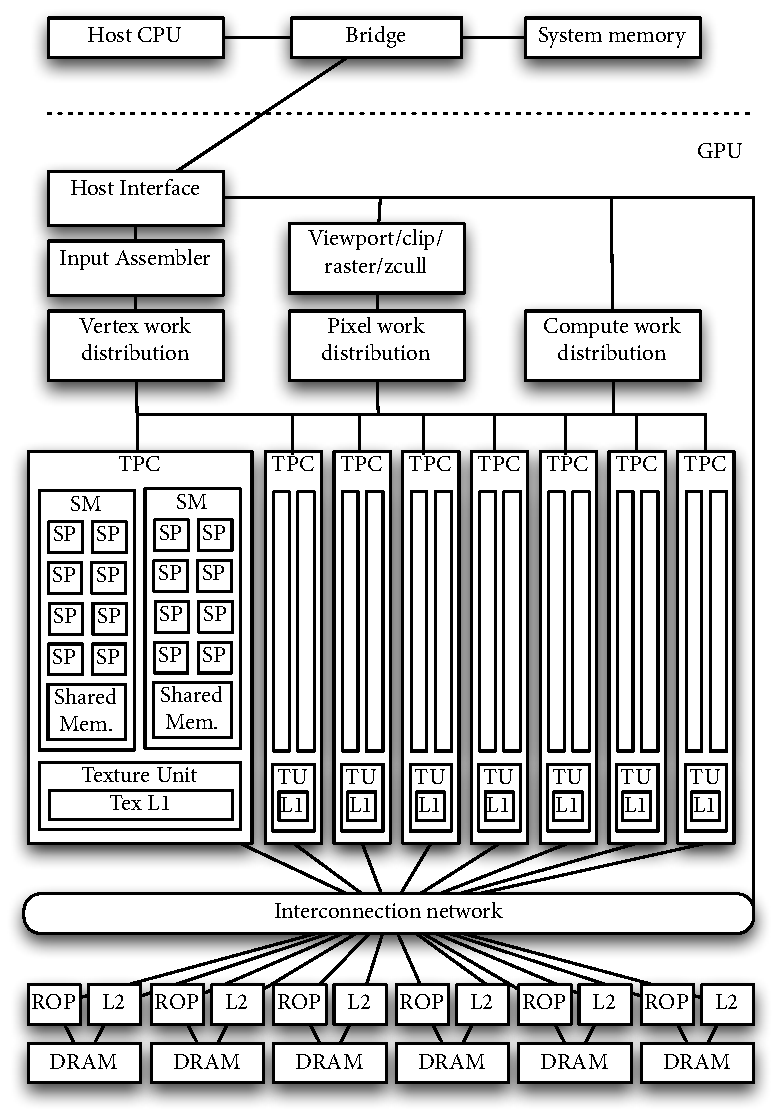
\includegraphics[width=0.6\textwidth]{gfx/tesla_architecture}
\caption{Tesla Architecture}
\label{fig:itesla_architecture}
\end{figure}

The figure \autoref{fig:tesla_architecture} shows the Tesla architectures. As
mentioned above the new \gls{GPU} architectures are a radical departure
from traditional \gls{GPU} design (USM). The Tesla 8 Series has 16 multiprocessors. 
Each multiprocessor is composed of 8 streaming processors, 128 processors in 
total. Each streaming multiprocessor has 16 KB of shared memory
and a L1 cache attached and has access to a texture unit. A streaming processor
consists of a scalar ALU and performs floating point operations. 32 streaming
processor build up a \gls{SIMD} unit (warp) in that one instruction is executed.
The 8800 GTX has 768 MB of graphics memory, 620 GFlops of peak performance and
86 GB/s peak memory bandwidth. Many massively data-parallel algorithms can be
run sufficiently on this specialized architecture \citep{citeulike:3145468}.
Programming for this architecture is done with \gls{CUDA} (Common Unified Device
Architecture) the C language extension which will be covered in the next
section.
% section the_tesla_architecture (end)


\subsection*{Common Unified Device Architecture (CUDA)} % (fold)
\label{sub:icommon_unified_device_architecture_cuda_}
In 2007, {\slcsmallcaps{NVIDIA}} introduced an extended ANSI C programming model and software
environment the Compute Unified Device Architecture (CUDA). The reason why CUDA
was is born is that parallelism is increasing rapidly with Moore's
law\footnote{Processor count is doubling every 18 - 24 months} and the challenge
is to develop parallel application software that scales transparently with the
number of processor cores. The main goals when \gls{CUDA} was developed were that it
scales to 100s of cores, 1000s of parallel threads and it allows heterogeneous
computing (CPU + GPU). All this considerations led to the result that \gls{CUDA} runs
on any number of processors without recompiling an the parallelism applies to
both \glspl{CPU}and \glspl{GPU}\citep{citeulike:3839013}.

CUDA is C with minimal extensions and defines a programming and memory model.
There are three key abstractions in CUDA, a hierarchy of thread groups, shared
memories and barrier synchronization \citep{citeulike:3325943} that are exposed
to the developer. \gls{CUDA} uses extensive multithreading where threads express
fine-grained instruction, data and thread parallelism that are grouped into
thread blocks which express coarse grained data and task parallelism. The
developer has to rethink about his algorithms to be aggresively parallel.
The problem has to be split into indepedent coarse sub-problems and at finer
level into fine-grained sub-problems that can be solved cooperatively
\citep{citeulike:3325943}.

CUDA has been accepted be many developers which can be seen by the huge amount
of already developed software and contributions to the \gls{CUDA} Zone:
\emph{www.nvidia.com/cuda}. A brief look shows the \gls{CUDA} computing sweet 
spots\citep{citeulike:3839013}: 
\begin{itemize} 
	\item High arithmetic intensity (Dense linera algebra, PDEs, n-body, 
			finite difference, \ldots) 
	\item High bandwidth Sorting, database, sequencing, virus scanning, genomics, \ldots) 
	\item Visual computing: (Graphics, image processing, tomography, 
			machine vision, \ldots) 
	\item Computational modeling, science, engineering, finance, ... 			
\end{itemize}

This is just a small snapshot of algorithms that can be used with \gls{CUDA} on
GPUs. For a more extensive list and speedups compared to high end CPUS see
\emph{www.nvidia.com/cuda} and \emph{www.gpGPU.org}.
 % section common_unified_device_architecture_cuda_ (end)

\subsection*{CUDA Programming Model} % (fold)
\label{sub:icuda_programming_model}
The \gls{CUDA} programming model exposes the graphics processor as a highly
multithreaded coprocessor. The graphics processor is viewed as a compute device
that is a coprocessor to the host that has its own device memory and runs many
threads in parallel.

Applications are accelerated by executing data parallel portions of the
algorithm on the \gls{GPU} as \emph{kernels} which run in parallel on
many threads. There are some major differences between CPU and \gls{GPU} threads. 
A \gls{GPU} needs thousands of threads for full efficience where \glspl{CPU} only need a few of
them. \gls{GPU} threads have a very little creation overhead and are extremely
lightweight compared to CPU threads.

\paragraph{Thread Batching} % (fold)
\label{par:ithread_batching}
A kernel is executed as a grid of thread blocks where data memory space is
shared by all threads. A thread block is a batch of threads that can cooperate
with each other by synchronizing there execution\footnote{For hazard free shared
memory access} and efficiently sharing data through the low latency shared
memory. Two threads from two different blocks can cooperate with atomic 
functions through the global memory. The identification of a thread is 
accomplished through block and thread ids which are assigned to each thread at 
creation time. 
% paragraph thread_batching (end)

\paragraph{Block and Thread IDs} % (fold)
\label{par:iblock_and_thread_ids}
Every thread and block have a unique id. As a result of this each thread can
decide whata data to work on. For every block there is a assigned id in 1D or 2D
layout. Thread ids can be accessed either with 1D, 2D or 3D coordinates similar
to multidimensional arrays. It simplifies memory addresing when processing
multidimensional data. For example image processing, matrix multiplication or
solving partial differential equations on volumes and so on. The data can reside
in several levels of the device memory. 
% paragraph block_and_thread_ids (end)

\paragraph{Device Memory Space} % (fold)
\label{par:idevice_memory_space}
The memory space is a hierarchy of several memory types that can be accessed per
thread, block, grid and the host. The threads have access to all memory levels
beginning with the read/write (rw) registers, local, shared, global, read only
(ro) texture and constant memory. The grids have only access to global, constant
and texture memory. Whereas the CPU (host) can (rw) global, constant and texture
memories.

Global, constant and texture memory have long latency accesses. They reside off
chip where registers local\footnote{Not true for older \glspl{GPU}chips where local
data is spilled out to global memory} and shared memory reside on-chip. The
global, constant and texture memory are mainly used for communication of (rw)
data between host and device where the contents is visible to all threads. As
mentioned above texture and constant memory can be written by the host where
constants and textures are initialized.
% paragraph device_memory_space (end)


\subsection*{A Simple Example} % (fold)
\label{sub:ia_simple_example}
This simple example will show the structure of an \gls{CUDA} program. The executing
kernel will do some easy calculations on the data provided, load the data into
shared memory  and write back the results to the global memory. 

A \gls{CUDA} program has a specific structure where the major parts are described in
this paragraph. The first thing to do is to initialize the device and some
auxiliary variables. THe \autoref{lst:iinit} shows the initalization.

%
\begin{lstlisting}[caption=Hardware initalization, label=lst:iinit]
int main( int argc, char** argv) {
	CUT_DEVICE_INIT(argc, argv);

	uint32_t num_threads = 32;
	uint32_t mem_size = sizeof(float) * num_threads;
	    							
                  ...
\end{lstlisting}
%

Since the \gls{GPU} is attached to the PCIe bus the host has no direct access to 
the global, constant and texture memory and has to transfer the data back
and forth with the DMA engine of the device. This is accomplished through the 
CUDA api calls that initiate the transfer. Before any transfer can be done
one has to allocate memory on the host and on the device for input and output
data. This is shown in listing \autoref{lst:idatatransfer}.


\begin{lstlisting}[caption=Data transfer of data, label=lst:idatatransfer]
	// allocate host memory 
	float* h_idata = (float*) malloc(mem_size);
	// allocate device memory 
	float* d_idata; cudaMalloc((void**) &d_idata, mem_size);
	// allocate device memory for result
	float* d_odata; cudaMalloc((void**) &d_odata, mem_size);
	// allocate mem for the result on host side
	float* h_odata = (float*) malloc( mem_size);
	// copy host memory to device 
	cudaMemcpy(d_idata, h_idata, mem_size, cudaMemcpyHostToDevice);
\end{lstlisting}


After setting up the input data the setup execution parameters are defined that
are used to startup the kernel. The $grid(1, 1, 1)$ statement defines a
multi-dimensional array of grids $x=1, y=1, z=1$ whereas the
$threads(num\_threads, 1, 1)$ defines a multi-dimensional array of threads
$x=num\_threads, y=1, z=1$ which are actually $1D$ arrays. Listing
\autoref{lst:iexecution} shows the call of the kernel with its input and output data.


\begin{lstlisting}[caption=Execution of the Kernel, label=lst:iexecution]
	    // setup execution parameters
	    dim3  grid( 1, 1, 1);
	    dim3  threads(num_threads, 1, 1);

	    // execute the kernel
	    kernel<<< grid, threads, mem_size >>>(d_idata, d_odata);

\end{lstlisting}



If everything went well the host can copy the data from device memory
to host memory and check, visualize or store the calculated values. Listing
\autoref{lst:iresult} shows the last steps before exiting the program.


\begin{lstlisting}[caption=Retrieving of the Results, label=lst:iresult]
	    // check if kernel execution generated and error
	    CUT_CHECK_ERROR("Kernel execution failed");
 
	    // copy result from device to host
	    cudaMemcpy(h_odata, d_odata, sizeof( float) * num_threads, 
			       cudaMemcpyDeviceToHost);

	    // cleanup memory free(x), free(y), free(z) ...
		CUT_EXIT(argc, argv);
	}
\end{lstlisting}



The previous listings showed the host code and how to launch a kernel on the
device. The listing \autoref{lst:idevice} shows the device code portion. There are
several qualifiers that define which function is compiled for which processing
unit. The \textit{\_\_global\_\_} qualifier specifies that this function is run
on the device and hence compiled for the \gls{GPU} where the \textit{\_\_host\_\_}
qualifier specifies that this function is only run on the host and not on the
device. There are more function specifiers that can be looked up in
\citep{citeulike:3325943}.

For data there are as well qualifiers where one can specify where the data is
located, either in constant, global or shared memory. In listing
\autoref{lst:idevice} the \textit{\_\_shared\_\_} qualifier is used. The device will
use the shared memory to preload the data for faster access.


\begin{lstlisting}[caption=CUDA device code, label=lst:idevice]
	#include <stdio.h>

	#define SDATA(index) CUT_BANK_CHECKER(sdata, index)
	// Simple test kernel for device functionality
	__global__ void kernel( float* g_idata, float* g_odata) 
	{
	  // shared memory
	  // the size is determined by the host application
	  extern  __shared__  float sdata[];

	  // access thread id
	  const unsigned int tid = threadIdx.x;
	  // access number of threads in this block
	  const unsigned int num_threads = blockDim.x;

	  // read in input data from global memory
	  // use the bank checker macro to check for bank conflicts during host
	  // emulation
	  SDATA(tid) = g_idata[tid];
	  __syncthreads();

	  // perform some computations
	  SDATA(tid) = (float) num_threads * SDATA( tid);
	  __syncthreads();

	  // write data to global memory
	  g_odata[tid] = SDATA(tid);
	}

\end{lstlisting}


After loading the data the kernel just multiplies the thread-id with the number
of threads and saves the result back to global memory where the host can pick up
the result.
% section a_simple_example (end)
% section cuda_programming_model (end)
% section background_to_the_project (end)


\section*{Initial Survey} 
\label{sub:iinitial_survey} 
% This survey is a quick perliminary survey, to discover something of the shape 
% of the relevant field of information; in doing this you will identify key 
% abstracts, journals, books, series of reports, and so on. Key technical issues 
% will be summarised.
The first thing to answer is why should someone do general purpose computing on
GPUs (GPGPU) anyway. For the most people \glspl{CPU}are just enough. They do not
demand on high computational power and on a high bandwidth. Still there is
paradigm shift taking place and this can not be neglected. As stated in
\citep{citeulike:1187394} and in \citep{citeulike:3421647} CPU manufacturers are
facing problems which they cannnot overcome just by increasing the frequency.
The often cited \emph{Walls} are first, \emph{The Memory
Wall}\citep{citeulike:457955}, \emph{The Frequency Wall} and \emph{The Power
Wall}. The only way seen by CPU makers is currently to go multicore. Intel e.g.
went multicore with there new \emph{Core Microarchitecture} for consumer
products and even a \gls{GPU} replacement, \emph{Larrabee} \citep{citeulike:3153758}.
IBM, Toshiba and Sony developed the \emph{Cell Broadband Architecture} a 9 core
chip \citep{citeulike:1243173}. SUN developed the \emph{Niagara} CPU a multi-core
general purpose processor. It has eight in-order cores, each of them capable of
executing four simultaneous threads \citep{citeulike:3743958}.

Compared to \glspl{CPU}GPUs went years ago to multicore and multithreading. \glspl{GPU}are
maybe the kind of processor where \glspl{CPU}are heading to in terms of multithreading
and raw performance. Forecasts project that every two years the amount of cores
can double. The multicore approach may be the answer to the problems stated
above but this yields to another thing the \emph{parallel programming problem}
\citep{citeulike:3750573}. User will only benefit from this growth if software
can make use of all the cores. Many developers learned about the
single-threaded von neumann model and are not familiar with parallel code which
is subject to errors such as deadlocks and livelock, race conditions and many
more. Parallel programming is difficult and there are several paradigms to make
life easier for developers. 

On of these is the data-parallel paradigm. Where one
is not trying to assign diffferent subtasks to separate cores rather assigning
an individual data element to a separate core for processing
\citep{citeulike:3750565}. 3D rendering, an embarassingly data-parallel problem,
has driven the \gls{GPU} evolution which makes the \gls{GPU} a perfect target for
data-parallel code. There are several fine-grained or data-parallel programming
environments that leverage the \gls{GPU} for general purpose computing (Brook, Sh,
RapidMind, ...). 

The focus of this work will be CUDA\footnote{www.nvidia.com}. \gls{CUDA} is the only
environment which is not based on a graphics library and officialy released by
{\slcsmallcaps{NVIDIA}} for their GPUs. \gls{CUDA} is a minimal extension to C and C++ programming
languages. The technique employed by \gls{CUDA} is single process, multiple data
(SPMD). Tasks are split up and run simultaneously on multiple threads (cores)
with different input \citep{citeulike:3072519}.

\subsection*{Choosing a Fast Algorithm} % (fold)
\label{ssub:ichoosing_a_fast_algorithm}
Before even digging into the wide field of algorithms and difficult problems in
high performance computing one has to understand the hardware architecture of
the \glspl{GPU}to make a decision if an algorithm can be mapped on GPUs. A pretty good
overview over the {\slcsmallcaps{NVIDIA}} \gls{GPU} gives the \emph{{\slcsmallcaps{NVIDIA}} \gls{CUDA} Programming Guide}
\citep{citeulike:3325943}. A little bit outdatet but still of interest is
\emph{The GeForce 6 Series \gls{GPU} Architecture}\citep{citeulike:3757915} which gives
an overview how the \gls{GPU} fits into the whole system, what a fragment processor,
vertex processor or what textures are. To have a even deeper look into \glspl{GPU}the
article \citep{citeulike:2790995} is highly recommended.

\paragraph{Computations which Map Well to GPUs} % (fold)
\label{par:icomputations_which_map_well_to_GPUs}
It is important to understand that \glspl{GPU}are good at running computer graphics
and algorithms which \emph{mimic} or have the attributes of computer graphics in
terms of data parallelism and data independence. Not only that similar
computations are applied to streams of many data elements (vertices, fragments,
...) but also the computation of each element is completely or almost completely
independent \citep{citeulike:3733428}. Such types of algorithms are often called
embarassingly parallel algorithms where subtasks rarely or never communicate to
each other.

Another important fact for a algorithm is the \emph{Arithmetic Intensity}. The
Arithmetic Intensity is the ratio of computation to bandwidth or formally:
\begin{center} 
 \emph{arithmetic intensity = operations / words transferred.}
\end{center}
This fact is important because the increase of computational throughput is
faster than the memory throughput which leads to the problem known as \emph{The
Memory Wall}. \gls{GPU} memory systems are architected to deliver high bandwidth,
rather than low-latency, data access. As such computations that benefit most of
the \glspl{GPU}have a high arithmetic intensity \citep{citeulike:3733428}. The next 
sections will represent some algorithms which could fit to GPUs. 
% paragraph computations_which_map_well_to_GPUs (end)

\paragraph{Ray Tracing} % (fold)
\label{par:iray_tracing}
Ray Tracing \citep{citeulike:841961} is an embarrassingly parallel alorithm which
could fit well to GPUs. The author has a extensible knowledge of Ray Tracing on
massively parallel computers \citep{citeulike:80546}. Thats why Ray Tracing was
first considered for porting to the GPU. Unfortuneately there were several
implementations already done for the GPU. Nevertheless equipped with all the
knowledge about Ray Tracing and how to split up the work, arrange the data on a
parallel machine to run efficiently the Ray Tracing algorithm
\citep{citeulike:3770900} will be used for initial benchmarks and the feasibility
study.
% paragraph ray_tracing (end)

\paragraph{Photon Mapping} % (fold)
\label{par:iphoton_mapping}
Ray Tracing has a local illumination model. To generate more realistic effects
like caustics, diffuse / glossy indirect illumination and more a more
sophisticated model has to be used. Global illumination like \emph{Photon
Mapping} \citep{citeulike:635695} can create all the effects that Ray Tracing
cannot. There are implementations of photon mapping on GPUs
\citep{Purcell:2003:PMO} which are developed with graphics apis and not with
CUDA. Anyhow since photon mapping is heavily using a kd-tree it would be a major
effort to develop an efficient data structure which has the same functionality
as a kd-tree. Nevertheless the first candidate for porting to the \gls{GPU} is \emph{Photon Mapping}.
% paragraph photon_mapping (end)

\paragraph{Multiple Precision Arithmetic} % (fold)
\label{par:imultiple_precision_arithmetic}
Another interesting field which demands high computational power is number
theory. The most common/known application is asymmetric cryptography. To
decipher messages that are cyphered with an asymmetric algorithm one needs
superior computational power. An overview over common algorithms gives
\citep{citeulike:3783254}. All algorithms have one thing in common they need a
multiple precision library to represent numbers with 200 and more digits. A good
overview gives \citep{citeulike:3783244}.

The idea was to implement some of the factoring algorithms to the GPU. The only
thing needed is the multiple precision library. In \citep{citeulike:3783254} the
Gnu Multiple Precision (GMP) library was used to implement the algorithms. So
the multiple precision arithmetic is another candidate for porting to the GPU.
% paragraph multiple_precision_arithmetic (end)

\paragraph{High Dynamic Range} % (fold)
\label{par:ihigh_dynamic_range}
Image processing is always a candidate for embarassingly parallel algorithms. A
pretty new algorithm to enhance images is \emph{tone mapping}
\citep{citeulike:3783303}. Tone mapping is the compression of dynamics in High
Dynamic Range (HDR) pictures. There are several algorithms for tone mapping:
Mantiuk \citep{citeulike:3783315}, Reinhard \citep{citeulike:3783311}, Durand
\citep{citeulike:789299}, Fattal \citep{citeulike:3783313} and many more. All of
this algorithms are present in the pfs-tools library written by Krawczyk
\citep{citeulike:3783303}. As this document was written Krawczyk was already
implementing the pfs-tools on \gls{GPU} but not publishing it. Furthermore there is an
complete editor written for hdr image processing which is running on the GPU. So
HDR was discarded but there are several other algorithms in image processing
which are considered as candidates. Some algorithms in no particular order:
segmentation, tracking, filtering, ... and so on. This is put as another
candidate to the list of the possible algorithms for porting. 
%paragraphhigh_dynamic_range (end)

\paragraph{Genetic Algorithms} % (fold)
\label{par:igenetic_algorithms}
Parallel genetic algorithms are usually implemented on parallel machines but
fine-grained parallel genetic algorithms can be mapped to GPUs
\citep{citeulike:3801879}. In \citep{citeulike:3801866} its shown what kind of
genetic algorithm map well to \glspl{GPU}and how the work and communication is
handled. It is \emph{pretty} easy to implement simple genetic algorithms on the
GPUs but with increasing complexity one has to consider many more things: load
balancing, communication pattern, dynamic memory allocation, resolving of
recursion ... . Another paper \citep{citeulike:3801883} compares genetic
algorithms implemented on \glspl{CPU}and \glspl{GPU}and shows that the latter is much more
effective than the former. All genetic algorithms have one thing in common the
core algorithm. Once effectively implemented on the \gls{GPU} the core algorithm is
extended with definitions like the population, selection, recombination and
mutation to solve a specific problem. The skill here is to choose the right
definitions and not more the efficient implementation of the core algorithm. So
this topic excluded from the candidate list.
% paragraph genetic_algorithms (end)

\paragraph{Chaos Theory} % (fold)
\label{par:ichaos_theory}
Another interesting field is chaos theory. Especially the visualization of
chaos. The maybe most famous visualization of chaos is \emph{The Fractal Flames
Algorithm}. Fractal flames are a member of iterated function system class of
fractals created by Scott Draves \citep{citeulike:3801950}. He uses a rather
complicated set of functions in the system to generate stunning visualization of
the iterative process of the system. The next release will have support for the
GPU. Thats why it was firstly discarded but the research about chaos led to
other interesting papers respectively books.

There is no need to use approx. 21 function for a system to generate visually
appealing pictures of chaos. Sprott showed in \citep{citeulike:3745535} that even
with very simple functions one can create patterns in chaos. This patterns are
called \emph{Strange Attractors} and are the visualization of chaotic behaviour.
There are created by iterating a simple equation some million times. 

Pickover shows in his book \citep{citeulike:3812233} how to create patterns from
a variety of sources. He shows how to create nice looking patterns from fourier
analysis, acoustic, chemistry and many more. Anyhow all of these equations or
differential systems have on thing in common no matter how complicated the
system is the core algorithm is to iterate a specific equation with correct
input numbers to create chaos. The algorithm is heavily computational bound
which makes it a good candidate for porting to the GPU.
% paragraph chaos_theory (end)
% section choosing_a_fast_algorithm (end)
\subsection*{Summary} % (fold)
\label{ssub:isummary}
After examining many possible candidates which can be accelerated with an GPU,
some of them were already in progress, some other maybe not feasible in the
timeframe of a master thesis. Nevertheless one algorithm has to be chosen and
this specific one will be ported to the GPU.

By the means of this example the typical data parallel programming approach will
be shown and it will be illustrated how to think in paralllel.
% section summary (end)
% section initial_survey (end)
\section*{Aims and Objectives} 
\label{sub:iaims_and_objectives} 
% A clear statement of the Aims and Objectives. Remember, aims and objectives 
% are generally a statement of what is to be achieved, not how it is to be
% achieved.

% The aim gives you a general indication of what you might learn and how you
% might benefit from a course. However, it does not give you any details, or a
% means of assessing whether your learning has been successful. Objectives are
% used for this purpose.

One aim of this master thesis is to show whether graphic cards are suitable for 
general purpose computing. With an algorithm example that is running slow on a 
CPU the process of porting to a \gls{GPU} is examined. As a result, the algorithm
will be running by a magnitude faster on the GPU. 

Another aim is to understand the architecture and programming models of GPUs.
Therefore the algorithmic view to \glspl{GPU}will be presented and computational
concepts and efficient data structures explained. Understanding these key
concepts makes one understand the architecture of GPUs.

% The objectives tell you what you should be able to do after the course, eg on
% completion of this programme the learner will: 

% - be able to identify key principles of adult teaching and learning 
% - be able to apply educational techniques learned to everyday teaching and 
% supervision 
% have identified their own strengths and weaknesses in teaching and
% supervision. The objectives 
Dissasociation from sequential algorithms and thinking in parallel will be one
major discipline after working through this thesis. On will be able identify
algorithms that are well suited for \glspl{GPU}and design efficient data flow and high
performing code.

Assessment of algorithms, knowledge about \gls{GPU} architecture, program flow and
data access patterns make one able to rate if a \gls{GPU} is suitable for general
purpose computing.
% section aims_and_objectives (end)

\section*{Experimental/Investigative methods to be adopted} 
\label{ssub:iexperimental_investigative_methods_to_be_adopted} 
% An outline of the key activities necessary to complete the project, itemising
% the experimental methods to tebe used (in, for example, a design-based 
% project), or the investigative techniques to be adopted (in the case of, say, 
% a critical survey).
To estimate if an algorithm is suitable for running on the \gls{GPU} first of all the
hardware architecture has to be understood. Since \glspl{GPU}are \emph{completely}
different than \glspl{CPU}one has to understand how simple things like loops,
arithmetic, data access and program flow are managed on such hardware. The most
interesting part here is the fact that \glspl{GPU}are able to hold up to approx. 12000
threads in flight. Understanding the hardware is the key for high performance 
computing on GPUs.

To get an impression how one can/should write code for \glspl{GPU}a feasibility study
will be done that will show answers to statements stated above and further 
questions. 

Further questions arise when reading scientific papers about general purpose
computing on graphics hardware. Often there are statements which are not
applicable to current hardware generation. These limitation arise from the fact
that the \glspl{GPU}are implementing a graphics pipeline that is \emph{normally} used
for rasterization and rendering. The developers where confronted with an
graphics API and a graphics pipeline which thinks of triangles and pixel rather
than floats and integers. As a result the developers had to think about how to
rotate, scale or translate a triangle to perform a calculation in an algorithm.
There are several myths and truths about general purpose computing on graphics 
hardware which will be answered with the evolvment of the feasibility study. 

Since general purpose computing on graphics hardware is not more or less 'C'
programming with some extension, the best way to learn programming for \glspl{GPU}ist
learning by doing. Therefore several algorithms (Box Filter, Gaussian Blur, HDR,
... ) and further more will be studied.
This way one will get enough experience to structure a initial code and have
clue about how to split the work apart, offload computational intensive parts to
the \gls{GPU} and let do the general purpose processor the io and input handling.

Simple micro, synthetic\footnote{Synthetic benchmarks mimic a particular type of
workload on a component or system. Whereas application benchmarks run real world
programs} benchmarks are often used to describe the hardware by their peak
numbers. Either gflops achieveable or the bandwith between the processing unit
and the memory. They can easily show the basic conditions which one has to face 
with. Several benchmarks are already available in the SDK so only a few have to 
be developed. One critical point in general purpose computing is called
arithmetic density. Which describes how many arithmetic operations are executed
before another load is needed to fetch data. Micro benchmarks can easily show 
how arithmetic density effects performance, which in conclusion can show how 
performant an application will run on the GPU. 

The steps above will lead to a pretty good understanding of the hardware which
leads to the next step the searching and identifying a suitable algorithm to
port to the GPU. A critical survey of algorithms that are ported to \glspl{GPU}and
that are not ported will be done. There are many high performance algorithms out
there which take \emph{forever} to complete. If its chemistry, physics, biology,
astronomie and mathematics all of them can be ported to a \gls{GPU} to some extent. It
is important to fetch the applicable one and by means of that algorithm to show
the analysis and design process of high performance programs. There are
several things to consider when designing for parallel hardware which will be
examined an explained in the responsible chapters.

% section experimental_investigative_methods_to_be_adopted (end)
\section*{Time-plan} 
\label{sub:itime_plan} 
%Strongly related to the key activities identified above.
For the project \emph{General Purpose Computing on Graphics Hardware} the
following milestones were defined and listed below. Each milestone will have a
short description which tasks have to be accomplished to complete a mile stone.
With every milestone a chapter respectively a section of the master thesis will
be written which corresponds to the current carried out milestone. So the 
development of the milestones goes hand in hand with editing of the thesis.

\paragraph{M0: Interim Report (1/31/2009)} % (fold)
\label{par:iinterim_report}
For this milestone following tasks were done, the conduct of the initial survey 
and the writing of the interim report. The initial survey will give a coarse 
overview over the field and related work. 
% paragraph interim_report (end)

\paragraph{M1: Related Work Identified (2/14/2009)} % (fold)
\label{par:im1_related_work_identified}
The next step to take is to identify related work, conducting the literature 
survey. This survey should show the demand of GPGPU and used algorithms. 
Furhtermore it will help to understand the architecture and programming models. 
After gaining enough knowledge about the field its time to get the hands on the 
GPU.
% paragraph m1_related_work_identified (end)
\paragraph{M2: Algorithmic view understood (2/28/2009)} % (fold)
\label{par:im2_architecture_algorithmic_view_understood}
Equipped with the knowledge from the latter milestone it is time to understand
how the architecture works by examining algorithms already mapped to the GPU.
This step is crucial as it shows how algorithms map to and work on the \gls{GPU}
and a good understanding of the environment can help later on for choosing the
right algorithm for porting, analysis, design and implementation.
% paragraph m2_architecture_algorithmic_view_understood (end)
\paragraph{M3: Feasibility Study (3/14/2009)} % (fold)
\label{par:im3_feasibility_study}
The feasiblity study will be used for the first steps into GPGPU. A low featured
ray tracer will be used for examining what the hurdles and obstacles are when 
developing for the GPU. The knowledge will be used for choosing the right 
algorithm. 
% paragraph m3_feasibility_study (end)
\paragraph{M4: Application, Algorithm choosen (3/21/2009)} % (fold)
\label{par:im4_application_algorithm_choosen}
After completion of this milestone the algorithm is chosen to be ported to the 
GPU. So the next milestones will be concentrated only on this algorithm and not 
more generaly. 
% paragraph m4_application_algorithm_choosen (end)
\paragraph{M5: Analysis, Solution Proposed (4/4/2009)} % (fold)
\label{par:im5_analysis_solution_proposed}
Here a solution will be proposed and outstanding issues will be identified. 
There are several myths about GPGPU which will be stated here as well, because 
there are affecting the design of the application and cannot be discarded.
% paragraph m5_analysis_solution_proposed (end)
\paragraph{M6: Experiments (4/14/2009)} % (fold)
\label{par:im6_experiments}
To exclude all eventualities a set of experiments will be undertaken. This will 
as well solve all myths.
% paragraph m6_experiments (end)
\paragraph{M7: Design, Application Ported (5/14/2009)} % (fold)
\label{par:im7_design_application_ported}
This milestone will cover the design of the application with all constraints,
obstacles and hurdles that are involved with GPGPU. In this task the application
will be implemented and run on the GPU. A good implementation will need several
iterations were several aspects will be tuned: coalesced memory access, load
balancing and many more.
% paragraph m7_design_application_ported (end)
\paragraph{M8: Discussion (5/22/2009)} % (fold)
\label{par:im8_discussion}
Another important part is the discussion of the results and methodologies
applied which will be done in this milestone.
% paragraph m8_discussion (end)

\paragraph{M9: Master Thesis Edited (5/30/2009)} % (fold)
\label{par:imaster_thesis_edited}
Here the thesis will be recaped and briefly outlined. Conclusions will be drawn
and future work presented. A critical summary and conclusion will be provided as
well. % paragraph master_thesis_edited (end)

% section time_plan (end)
\section*{Deliverables or specific outcomes} 
\label{sub:ideliverables_or_specific_outcomes} 
% A clear statement of the expected outcome(s).
The main outcome of this work is to show how \glspl{GPU} can be utilized for general
purpose computing. There is a high demand on performance and computational power
for scientific algorithms. Developers search for new architectures to solve
problems in shorter time. One promising new architecture or hardware is the GPU.
Since years \glspl{GPU} were only used for rendering. The switch from fixed pipelines
to programmable pipelines let developers think about using \glspl{GPU}for general
purpose computing. Accidently thery were forced to use 3D apis
(OpenGL\footnote{http://www.opengl.org},
DirectX\footnote{http://www.microsoft.com}) to accomplish task like matrix
multiplication or fast fourier transformation. Nowadays developer use \gls{CUDA} or
middleware like RapidMind to develop software for ({\slcsmallcaps{NVIDIA}}) GPUs. It will be
shown that \gls{CUDA} is highly efficient and easy to program which makes general
purpose computing more feasible.

By the means of a application that is computationally intensive it will be shown
that traditional software engineering principles often do not apply to high
performance, parallel computing. Data access is the biggest problem of an
alogirthm to attain maximum performance. If the algorithm is memory bound and
not computational bound the limiting factor or bottleneck is the bandwidth to
the memory. Good data design is essential for good (performant) code. The data
and how it is used must be known in order to effectively design and optimize a
application for a \gls{GPU} or other highly parallel systems like the Cell processor
(Meine Diplomarbiet link). A simple computationally bound algorithm can be
easily designed in a way that it becomes memory bound if data arrangemnet and
access is neglected by the developer. The outcome of all the considerations will
be another approach how to tackle software design on such massively parallel
architecture.

Furthermore a workflow will be presented that shows how to port sequential code
to a massively parallel architecture. Software developer often only need to
compile their code with another compiler to \emph{port} the code to another
architecture. x86 -> PowerPC, x86 -> MIPS ... but the situation for parallel
processors like the cell, niagara and here the \gls{GPU} is completely different. One
has to identify the critical parts and explicitly offload tasks to the GPU. It
is obviuos that this is not the only step to do. Furthermore there are other
facts which have to be considered, like load-balancing, deadlocks, concurrency,
cache coherency and other. A workflow which can be adapted to different parallel
machines is another outcome of this work.

Last but not least is the outlook on future hardware development and programming
models. The problem with new hardware architectures is they have to be accepted
by the developers to succeed in industry. One way to achieve this is to have an
easy programming model which adapts easily to common apis and existing systems.
There are rarely branches of industry which want to, or are able to rewrite
their code for bleeding edge architectures like the cell or \glspl{GPU}if the outcome
is only 2x faster code. In this case many just extend their cluster with another
bunch of \emph{cheap} systems. A factor of 10 is an undocumented limit when to
invest in other, faster hardware.
% section deliverables_or_specific_outcomes (end)


%\chapter{Project Planning} % (fold)
\label{ch:project_planning}
\section*{Requirements} % (fold)
\label{sub:requirements}

% subsection requirements (end)

\section*{Scope of the Project} % (fold)
\label{sec:scope_of_the_project}
examine hardware and software stack by means of an algorithm which is used
to show the potential of GPU's for general purpose computing.
% subsection scope_of_the_project (end)

\section*{Milestone Plan (What to achieve)} % (fold)
\label{sec:milestone_plan_what_to_achieve_}
The following list shows the milestones that are identified by a 
brainstorming session and rationalized to a list of 15 - 25 milestones.

\begin{itemize}
	\item Interim report (see \autoref{ch:interim_report})
	\item Introduction, statement what the thesis is all about
	\item Related work identified (Literature reviewed)
	\item Algorithmic view understood
	\item Application choosen
	\item Solution proposal, outstanding issues identified
	\item Experiments undertaken, outstanding issues resolved. (Performance)
	\item Analysis of application
	\item Design of application
	\item Implementation of application
	\item Application ported
	\item Results and methodologies applied discussed
	\item Thesis recapped, briefly outlined, conclusion drawn and looked into future work
	% (Conclusion, questions, perspectives, summary. future work
\end{itemize}

% subsection milestone_plan_what_to_achieve_ (end)

\section*{Product Breakdown Structure (What to deliver)} % (fold)
\label{sec:product_breakdown_structure_what_to_deliver_}

% subsection product_breakdown_structure_what_to_deliver_ (end)

\subsection*{Work Breakdown Structure (What to do)} % (fold)
\label{sub:work_breakdown_structure}

% subsection work_breakdown_structure (end)

\subsection*{Organizational Breakdown Structure (Who does it)} % (fold)
\label{sub:organizational_breakdown_structure}

% subsection organizational_breakdown_structure (end)

% section project_planning (end)


%********************************************************************
% Other Stuff in the Back
%*******************************************************
\cleardoublepage\pagestyle{empty}

\hfill

\vfill


\pdfbookmark[0]{Colophon}{colophon}
\section*{Colophon}
This thesis was typeset with \LaTeXe\ using Hermann Zapf's
\emph{Palatino}
and \emph{Euler} type faces (Type~1 PostScript fonts \emph{URW
Palladio L}
and \emph{FPL} were used). The listings are typeset in \emph{Bera
Mono}, originally developed by Bitstream, Inc. as ``Bitstream Vera''.
(Type~1 PostScript fonts were made available by Malte Rosenau and
Ulrich Dirr.)

The typographic style was inspired by \cauthor{bringhurst:2002}'s genius as
presented in \emph{The Elements of Typographic Style} 
\citep{bringhurst:2002}. It is available for \LaTeX\ via \textsmaller{CTAN} as 
``\href{http://www.ctan.org/tex-archive/macros/latex/contrib/classicthesis/}%
{\texttt{classicthesis}}''.

\paragraph{note:} The custom size of the textblock was calculated
using the directions given by Mr. Bringhurst (pages 26--29 and
175/176). 10~pt Palatino needs  133.21~pt for the string
``abcdefghijklmnopqrstuvwxyz''. This yields a good line length between
24--26~pc (288--312~pt). Using a ``\emph{double square textblock}''
with a 1:2 ratio this results in a textblock of 312:624~pt (which
includes the headline in this design). A good alternative would be the
``\emph{golden section textblock}'' with a ratio of 1:1.62, here
312:505.44~pt. For comparison, \texttt{DIV9} of the \texttt{typearea}
package results in a line length of 389~pt (32.4~pc), which is by far
too long. However, this information will only be of interest for
hardcore pseudo-typographers like me.%

To make your own calculations, use the following commands and look up
the corresponding lengths in the book:
\begin{verbatim}
    \settowidth{\abcd}{abcdefghijklmnopqrstuvwxyz}
    \the\abcd\ % prints the value of the length
\end{verbatim}
Please see the file \texttt{classicthesis.sty} for some precalculated 
values for Palatino and Minion.

%    \settowidth{\abcd}{abcdefghijklmnopqrstuvwxyz}
%    \the\abcd\ % prints the value of the length


%\bigskip

%\noindent\finalVersionString





% ********************************************************************
% Game Over: Restart, Restore or Quit?
%*******************************************************
\end{document}
% ********************************************************************
